\documentclass[letterpaper, 11pt, colorful, sections]{cs1515}
\title{CSCI 1515: Applied Cryptography}
\author{P. Miao}
\date{Spring 2023}

\usepackage[textsize=tiny, textwidth=18mm]{todonotes}
\setuptodonotes{color=green!20}
\usepackage{marginnote}

\makeatletter
\renewcommand{\@todonotes@drawMarginNoteWithLine}{%
\begin{tikzpicture}[remember picture, overlay, baseline=-0.75ex]%
    \node [coordinate] (inText) {};%
\end{tikzpicture}%
\marginnote[{% Draw note in left margin
    \@todonotes@drawMarginNote%
    \@todonotes@drawLineToLeftMargin%
}]{% Draw note in right margin
    \@todonotes@drawMarginNote%
    \@todonotes@drawLineToRightMargin%
}%
}%
\makeatother

\usepackage{cancel}
\usetikzlibrary{cd}
\numberwithin{equation}{section}

\usepackage[all,cmtip]{xy}

\begin{document}
\maketitle
\begin{quote}
    \quad These are lecture notes for CSCI 1515: Applied Cryptography taught at \textsc{Brown University} by Peihan Miao in the Spring of 2023.

    \quad These notes are taken by Jiahua Chen with gracious help and input from classmates. Please direct any mistakes/errata\todo{FYI, todo's are marked like this.} to me via \href{mailto:jiahua_chen2@brown.edu}{email}, post a thread on Ed, or feel free to pull request or submit an issue to the notes repository (\url{https://github.com/BrownAppliedCryptography/notes}).

    \quad Notes last updated \today.
\end{quote}
\tableofcontents
% \bibliographystyle{alpha}
% \bibliography{bibliography}

\newpage
%!TEX root = ../notes.tex
\section{January 26, 2023}
\label{20230126}

\subsection{Introduction}
If you find a lot of courses on cryptography online or at universities, you'll find a lot of theoretical content. However, it's helpful for students to get hands-on experience with cryptography:
\begin{itemize}
    \item How cryptography has been used in practice,
    \item how cryptography will be used and implemented in the future.
\end{itemize}

The goal of this course is to

\emph{Introduction:} Peihan Miao, please refer by Peihan (you will be corrected if you address as professor). Joined Brown last semester, taught a seminar on research topic (Secure Computation). Before that, was in Chicago, and Visa Research even before that. Really loved math and theoretical computer science, started PhD with theoretical computer science. Shifted to applied side of cryptography; it's exciting to see cryptography implemented in practice. However, realized that most crypto courses are very theoretical---there are not a lot of courses that build up advanced applications using the tools that have been set up.

For this course, it will be \emph{much less} about math and proofs, and much more about how you can use these tools to do something more fun. It will be coding heavy, all projects will be implemented in C++ using crypto libraries. If, however, you are interested in the theoretical or mathematical side, you might consider other courses at Brown\footnote{CSCI 1510 and Math 1580 are good candidates. 1510 covers cryptographic proofs, and Math 1580 covers cryptography from a number theoretic perspective.}

\subsection{Course Logistics}
The course homepage is at \url{https://brownappliedcryptography.github.io/}.

\emph{Huge kudos to Nick and Jack for developing a new course from the ground up!}

\textbf{Please view the syllabus \href{https://docs.google.com/document/d/1SPlL17ee0XNtt4GF7FIcEp9pzA80lRHKfBE1bLBKImE/edit?usp=sharing}{here}. \emph{If there are differences between this document and the syllabus, the syllabus trumps this document.}}

The course is offered in-person in CIT 368, as well as synchronously over Zoom and recorded asynchronously (lectures posted online). You can do either\footnote{It is a 9AM class...} but try to attend online because there will be interaction! Lecture attendance is encouraged!

\textbf{EdStem} will be used for course questions, and \textbf{Gradescope} is used for assignments.

For assignments: \emph{Project 0} is a warmup for C++. Projects 1 \& 2 is to develop secure communication or authentication systems using the underlying cryptographic libraries. The later project, 3, 4 \& 5 will be on more advanced topics. The first 2 are more basic that are developed in practice, and the latter ones are more experimental in practice (so this is recent research in applied cryptography). The final project will be a combination of the existing projects or a project entirely new (separate from the earlier projects, but using the same cryptographic primitives).

Projects 1 through 5 will be accompanied with homework assignments (appropriately numbered 1 through 5) that develop a conceptual understanding of the materials.

Projects 1 \& 2 are to be done individually, the later projects are done in pairs (you can choose to go solo if you so wish as well). You are encouraged to find partners earlier on to discuss and work with them from the beginning. You are \emph{encouraged} to communicate with your partners on projects 1 \& 2 so you gain a conceptual understanding. You should complete your own write-up and code for the first two projects, however.

There is an option to capstone this course, contact Peihan about this. It would also be best to find a partner who is also capstoning this course.

The following is the grading policy:
\begin{center}
    \begin{tabular}{@{}ll@{}}
        \toprule
        \textit{Type}      & \textit{Percentage} \\ \midrule
        Project 0          & 5\%                 \\
        Projects 1 \& 2    & 20\% (10\% each)    \\
        Projects 3, 4 \& 5 & 45\% (15\% each)    \\
        Homeworks          & 20\% (2\% each)     \\
        Final Project      & 20\%                \\ \bottomrule
    \end{tabular}
\end{center}

You have 6 late days for \emph{projects}, of which at most two can be used on a single project. Additionally, you have 3 late days for \emph{homeworks}, of which at most one can be used on a single homework.

If you're sick, let Peihan know with a Dean's note.

\subsection{What is cryptography?}
...or more importantly, what is cryptography used for?

At a high level, \emph{cryptography is a set of techniques that protect information}.

\begin{ques*}
    What are some cryptographic techniques used in practice and what does it achieve?
\end{ques*}
\begin{itemize}
    \item Used in financial institutions.
          \begin{itemize}
              \item When you make a purchase, you might not want people to see your bank balance, what else you have purchased, etc.
          \end{itemize}
    \item Might be used in voting schemes. Making sure that ballots are kept private.
    \item Messaging systems, recently.
          \begin{itemize}
              \item End-to-end texting.
          \end{itemize}
    \item Storing medical records.
          \begin{itemize}
              \item More generally, any sensitive information.
              \item You don't want anyone else getting access to this sensitive information.
          \end{itemize}
    \item Used in military or war.
          \begin{itemize}
              \item Historically, it was used a lot in the military for secure communication.
          \end{itemize}
    \item Authentication systems. Login systems.
          \begin{itemize}
              \item There is authentication going on that ensures that \emph{only you} can log in.
          \end{itemize}
\end{itemize}

\subsection{Secure Communication}
We'll start with the most primitive of cryptography: \emph{secure communication}.

\begin{center}
    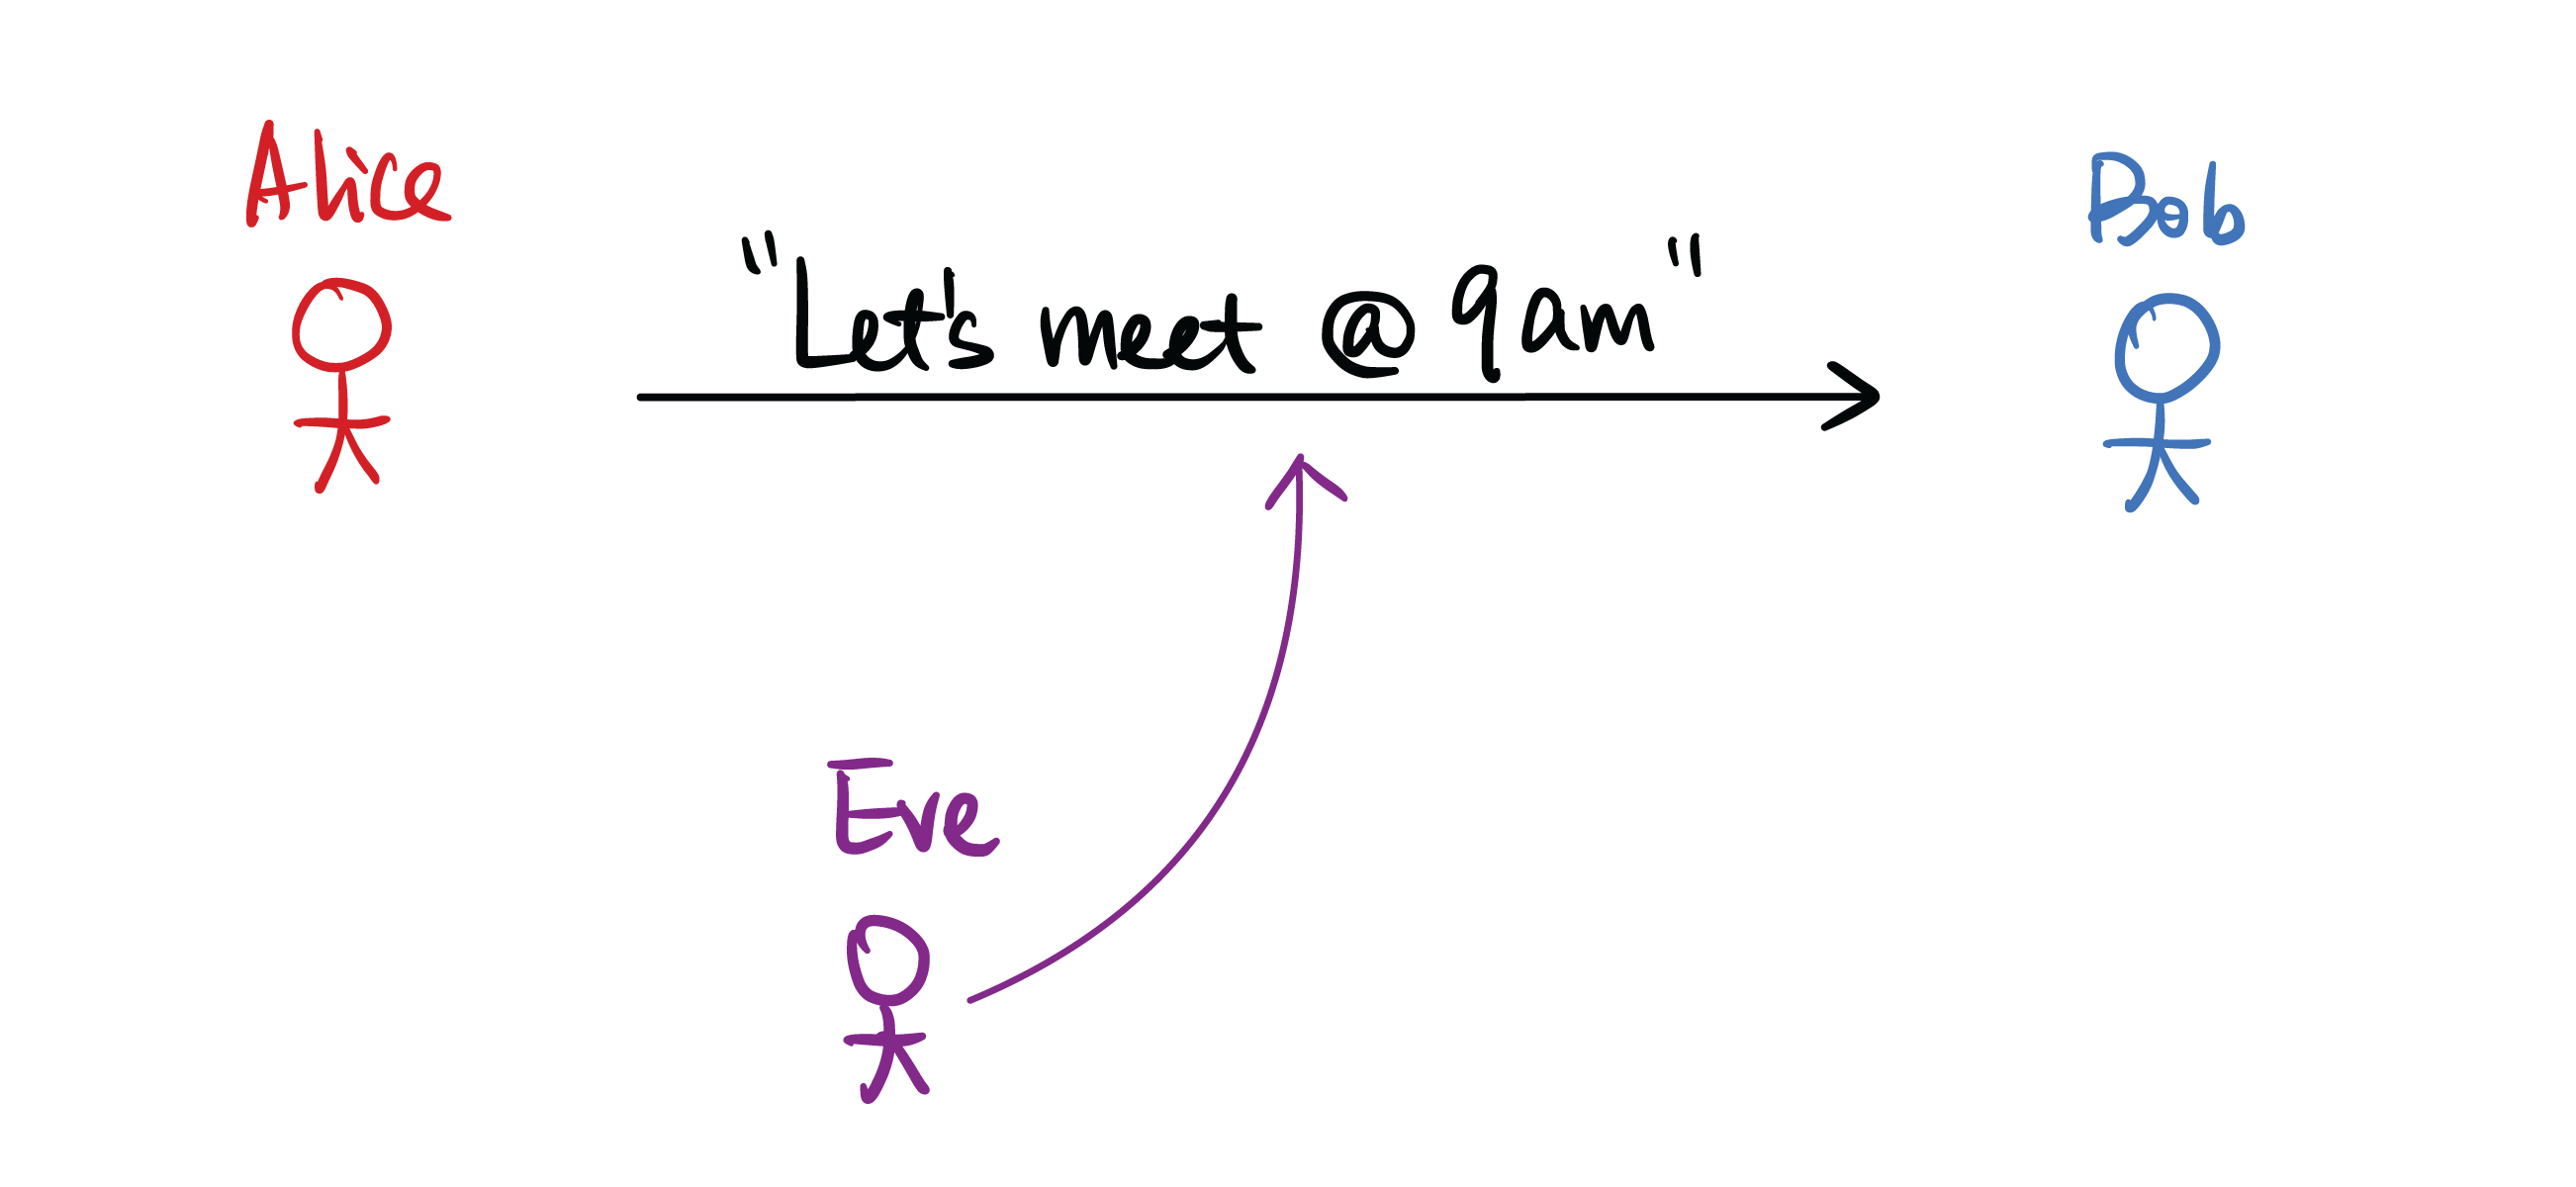
\includegraphics[width=0.8\textwidth]{images/2023-01-26/secure_computation.png}
\end{center}

Assume Alice wants to communicate to Bob ``Let's meet at 9am'', what are some security guarantees we want?

\begin{itemize}
    \item Eve cannot \emph{see} the message from Alice to Bob.
    \item Eve cannot \emph{alter} the message from Alice to Bob.
\end{itemize}

These two guarantees are the most important guarantees! The former is called \ul{message secrecy}, the latter is called \ul{message integrity}.

\subsubsection{Message Secrecy}

\begin{definition}[Message Secrecy]
    We want cryptography to allow Alice to \emph{encrypt} the message $m$ (which we call \emph{plaintext}) by running an algorithm that produces a \emph{ciphertext} $c$.

    Bob will be able to receive the ciphertext $c$ and run a \emph{decrypt} algorithm to produce the message $m$ again. This is akin to a secure box that Alice locks up, and Bob unlocks, while Eve does not know the message.

    \begin{center}
        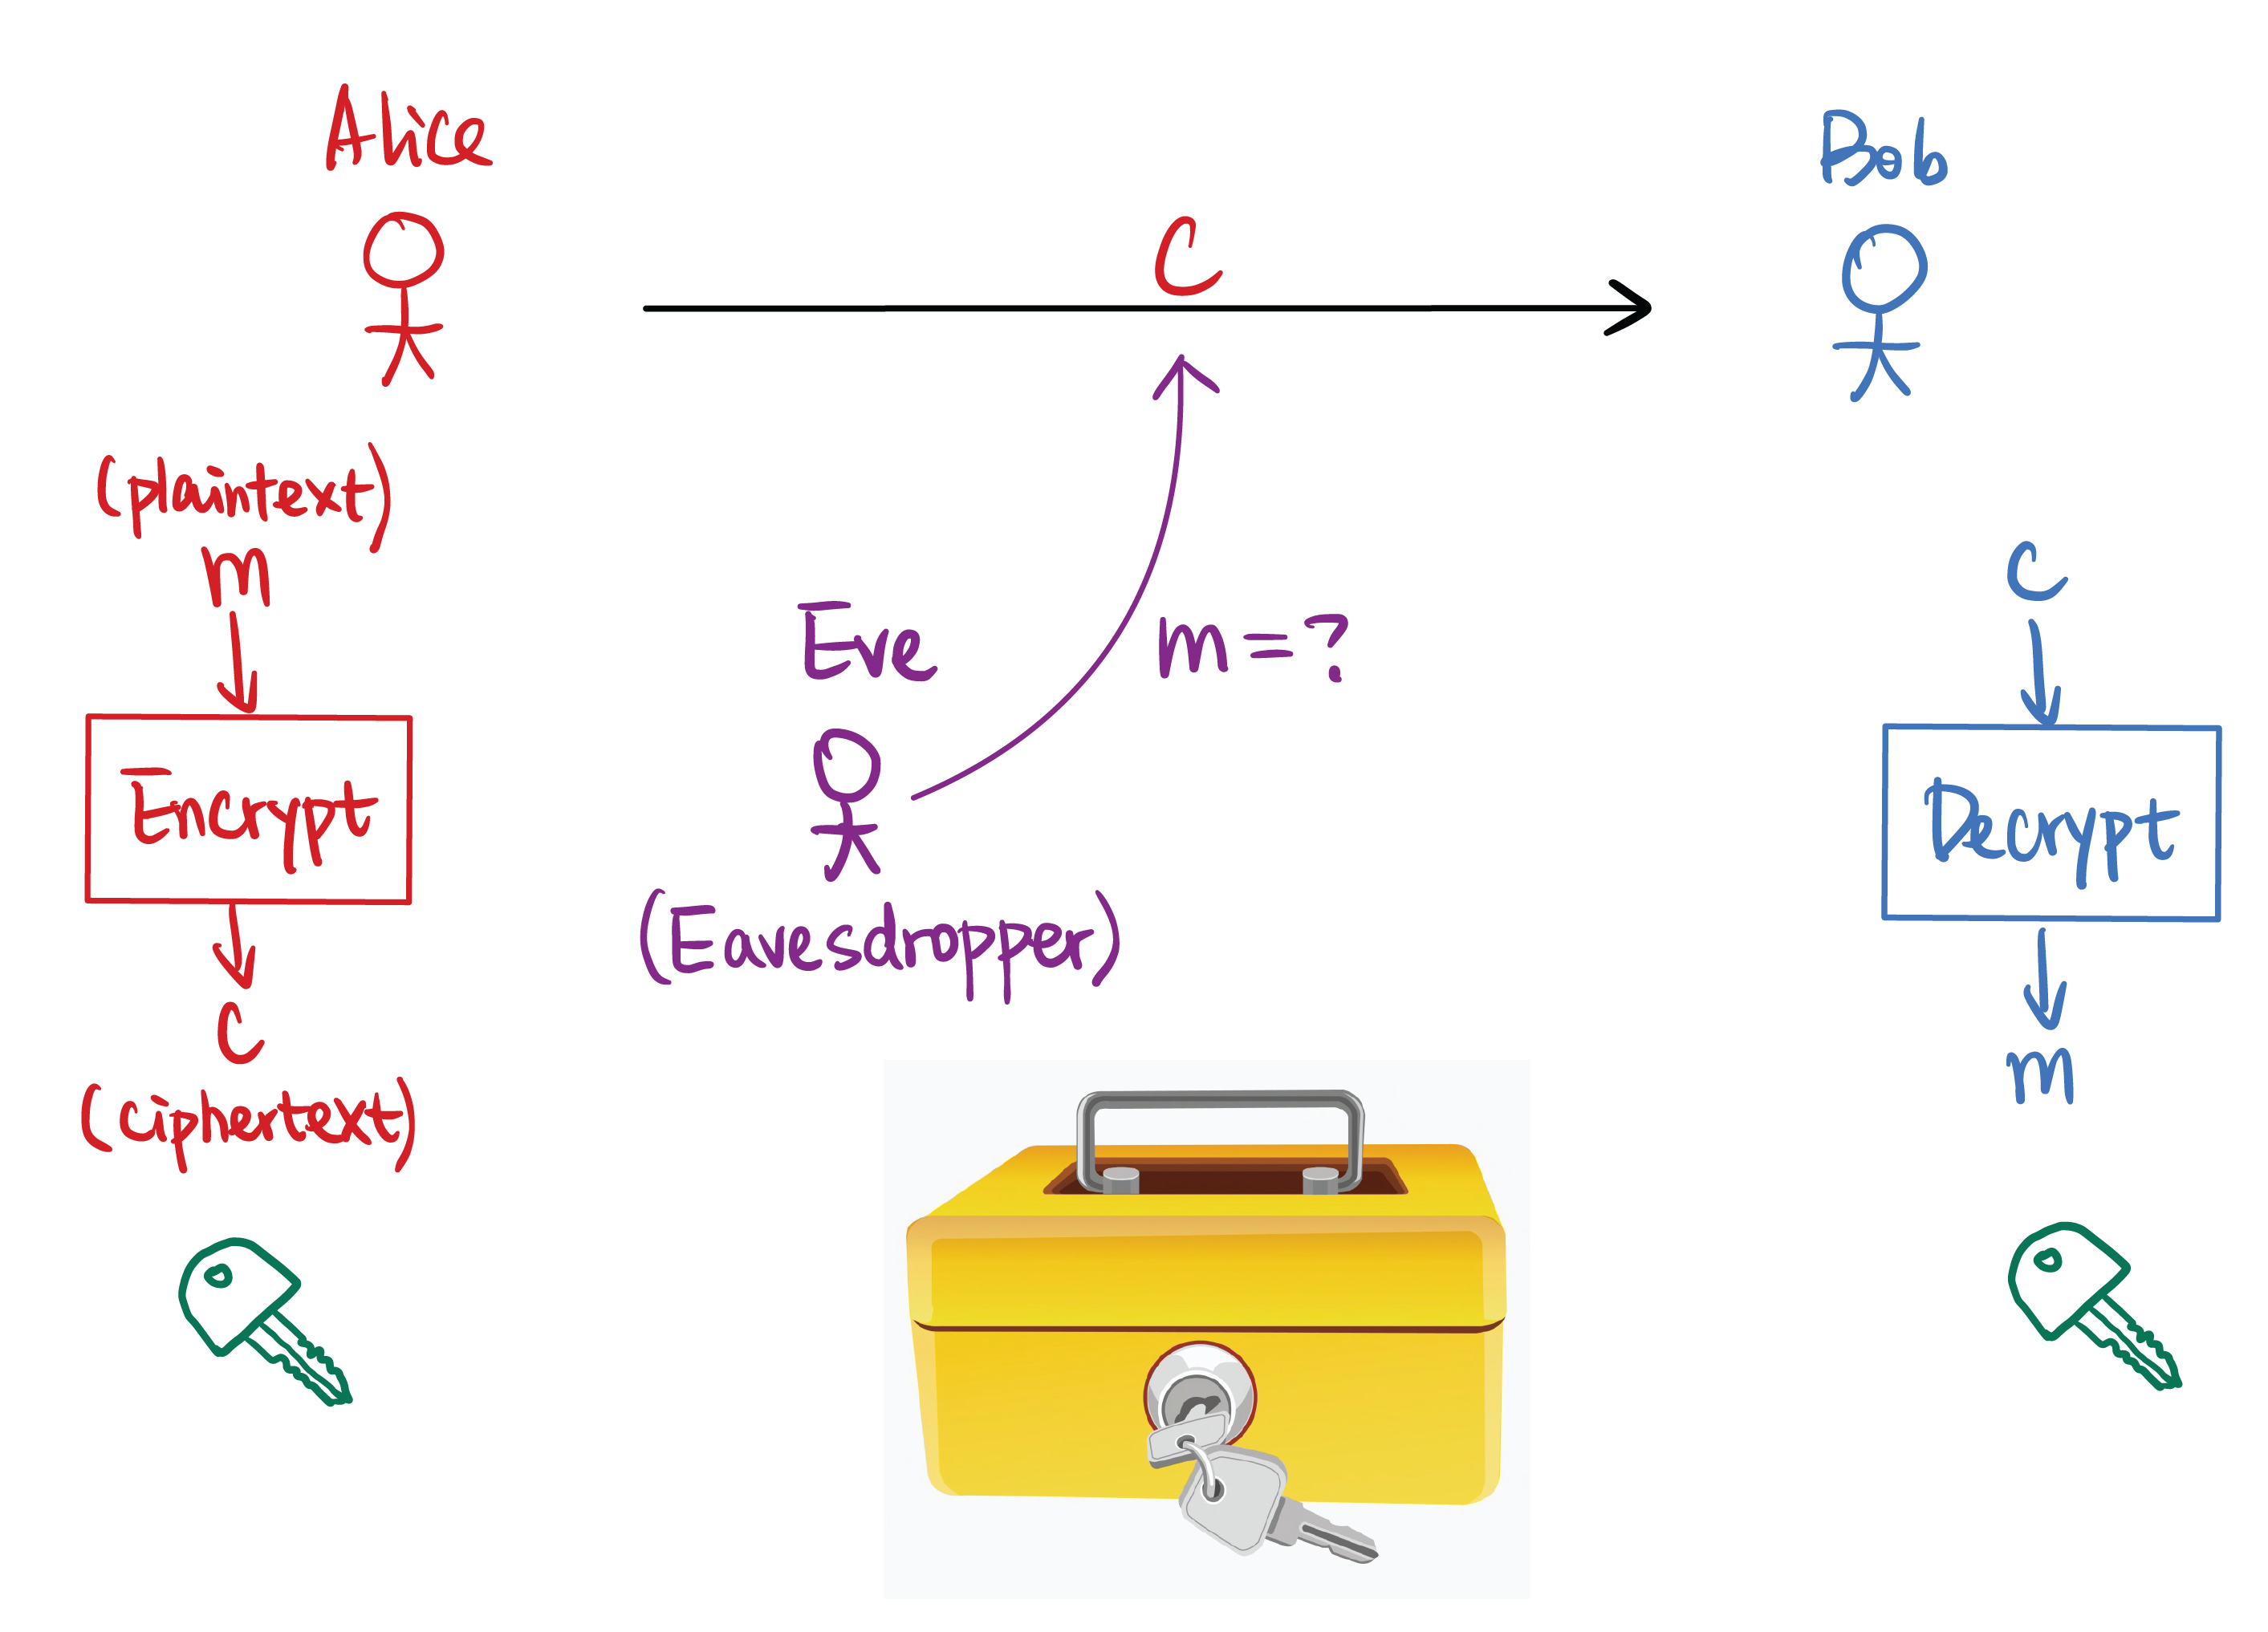
\includegraphics[width=0.8\textwidth]{images/2023-01-26/message_secrecy.png}
    \end{center}

    In this model, Eve is a weaker adversary, an \emph{eavesdropper}. Eve can only see the message, not alter it.
\end{definition}

\begin{example}[Substitution Cipher]
    The key that Alice and Bob jointly uses is a permutation mapping from $\{A\dots Z\}\to \{A\dots Z\}$. This mapping is the \emph{secret key}.

    Bob also has the mapping, and takes the inverse of the permutation to retrieve the message.

    \begin{center}
        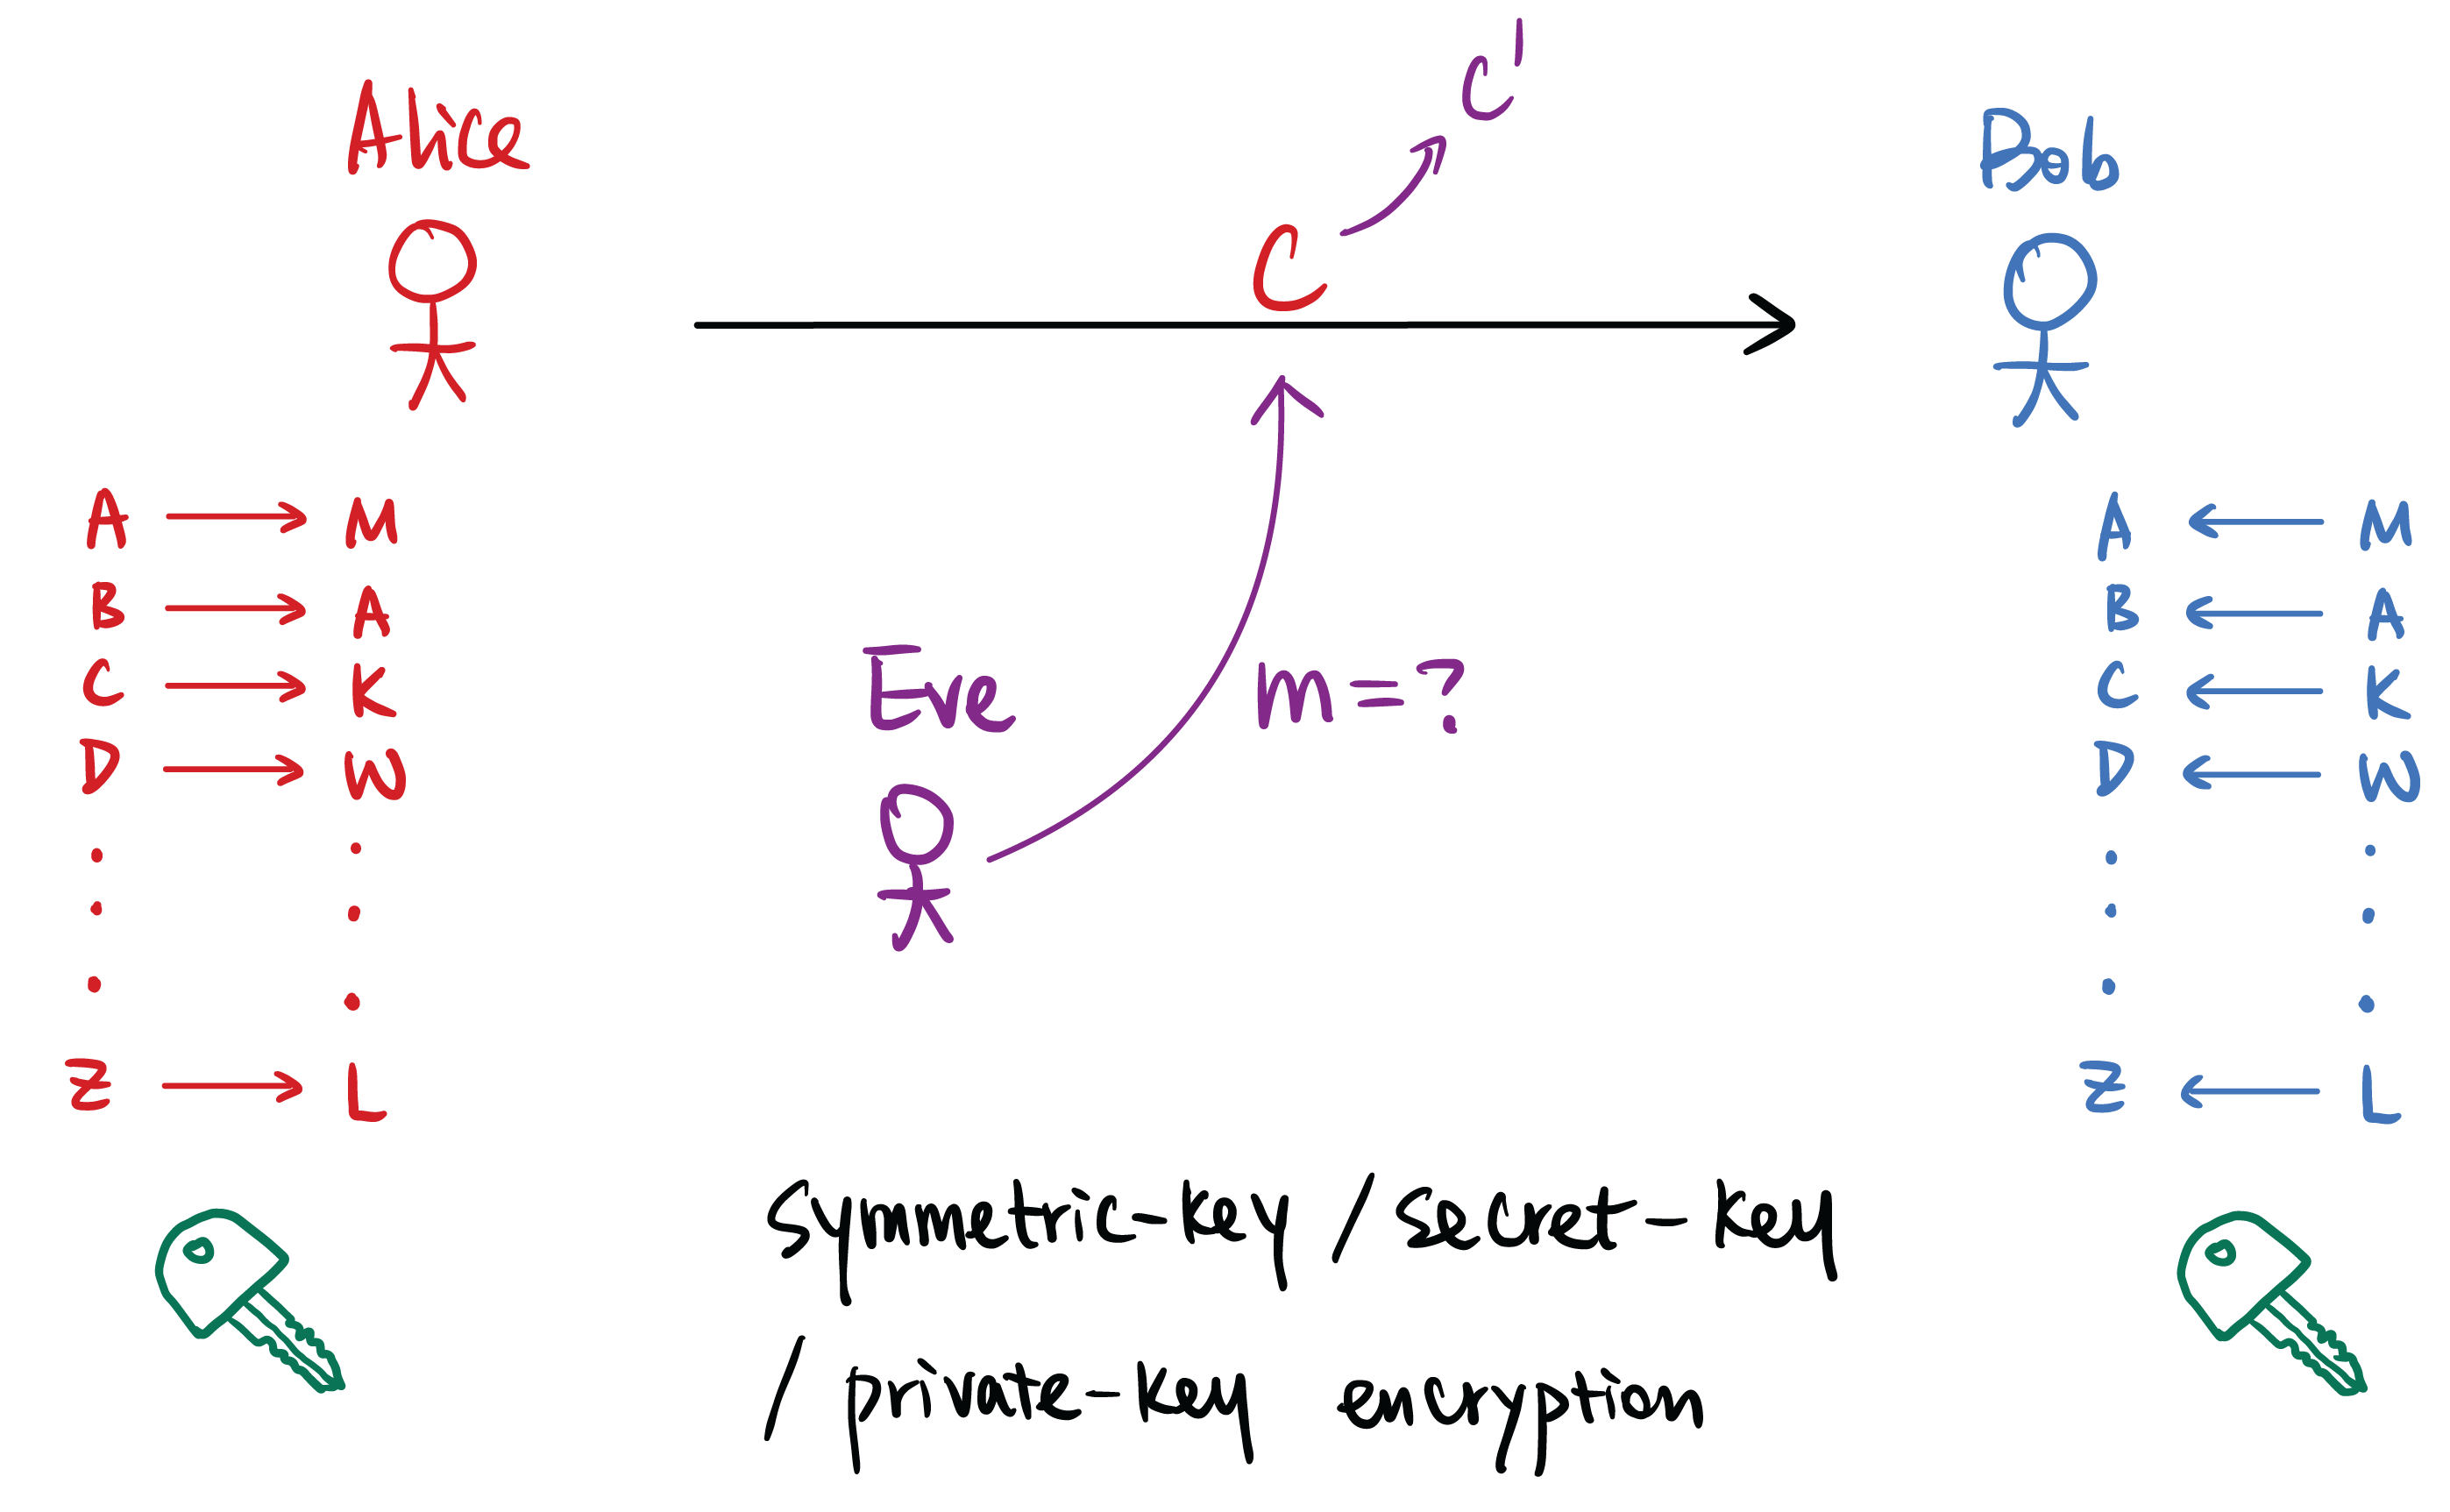
\includegraphics[width=0.9\textwidth]{images/2023-01-26/substitution_cipher.png}
    \end{center}

    This scheme is not quite secure! \emph{Why?}

    You could guess a bunch of vowels and see what words could make up. If you have a long enough message, you can see which letters appear more often. We know that in English, the vowels appear more often; and you can make a lot of guesses.
\end{example}
\begin{remark*}
    This encryption scheme also requires that Alice and Bob meet up in person to exchange this shared private key. Schemes like this are called \emph{symmetric-key, secret-key, or private-key encryption}. They need to meet up first to exchange secret keys.
\end{remark*}

\begin{definition}[Public-key Encryption]
    There is another primitive that is much more ideal/stronger, \ul{public-key encryption}. Bob publishes both a \emph{public} key and a \emph{private} key. You can consider a lock where you don't need a key to lock it\framedfootnote{You literally click it closed}, and only Bob has the key to unlock it.

    \begin{center}
        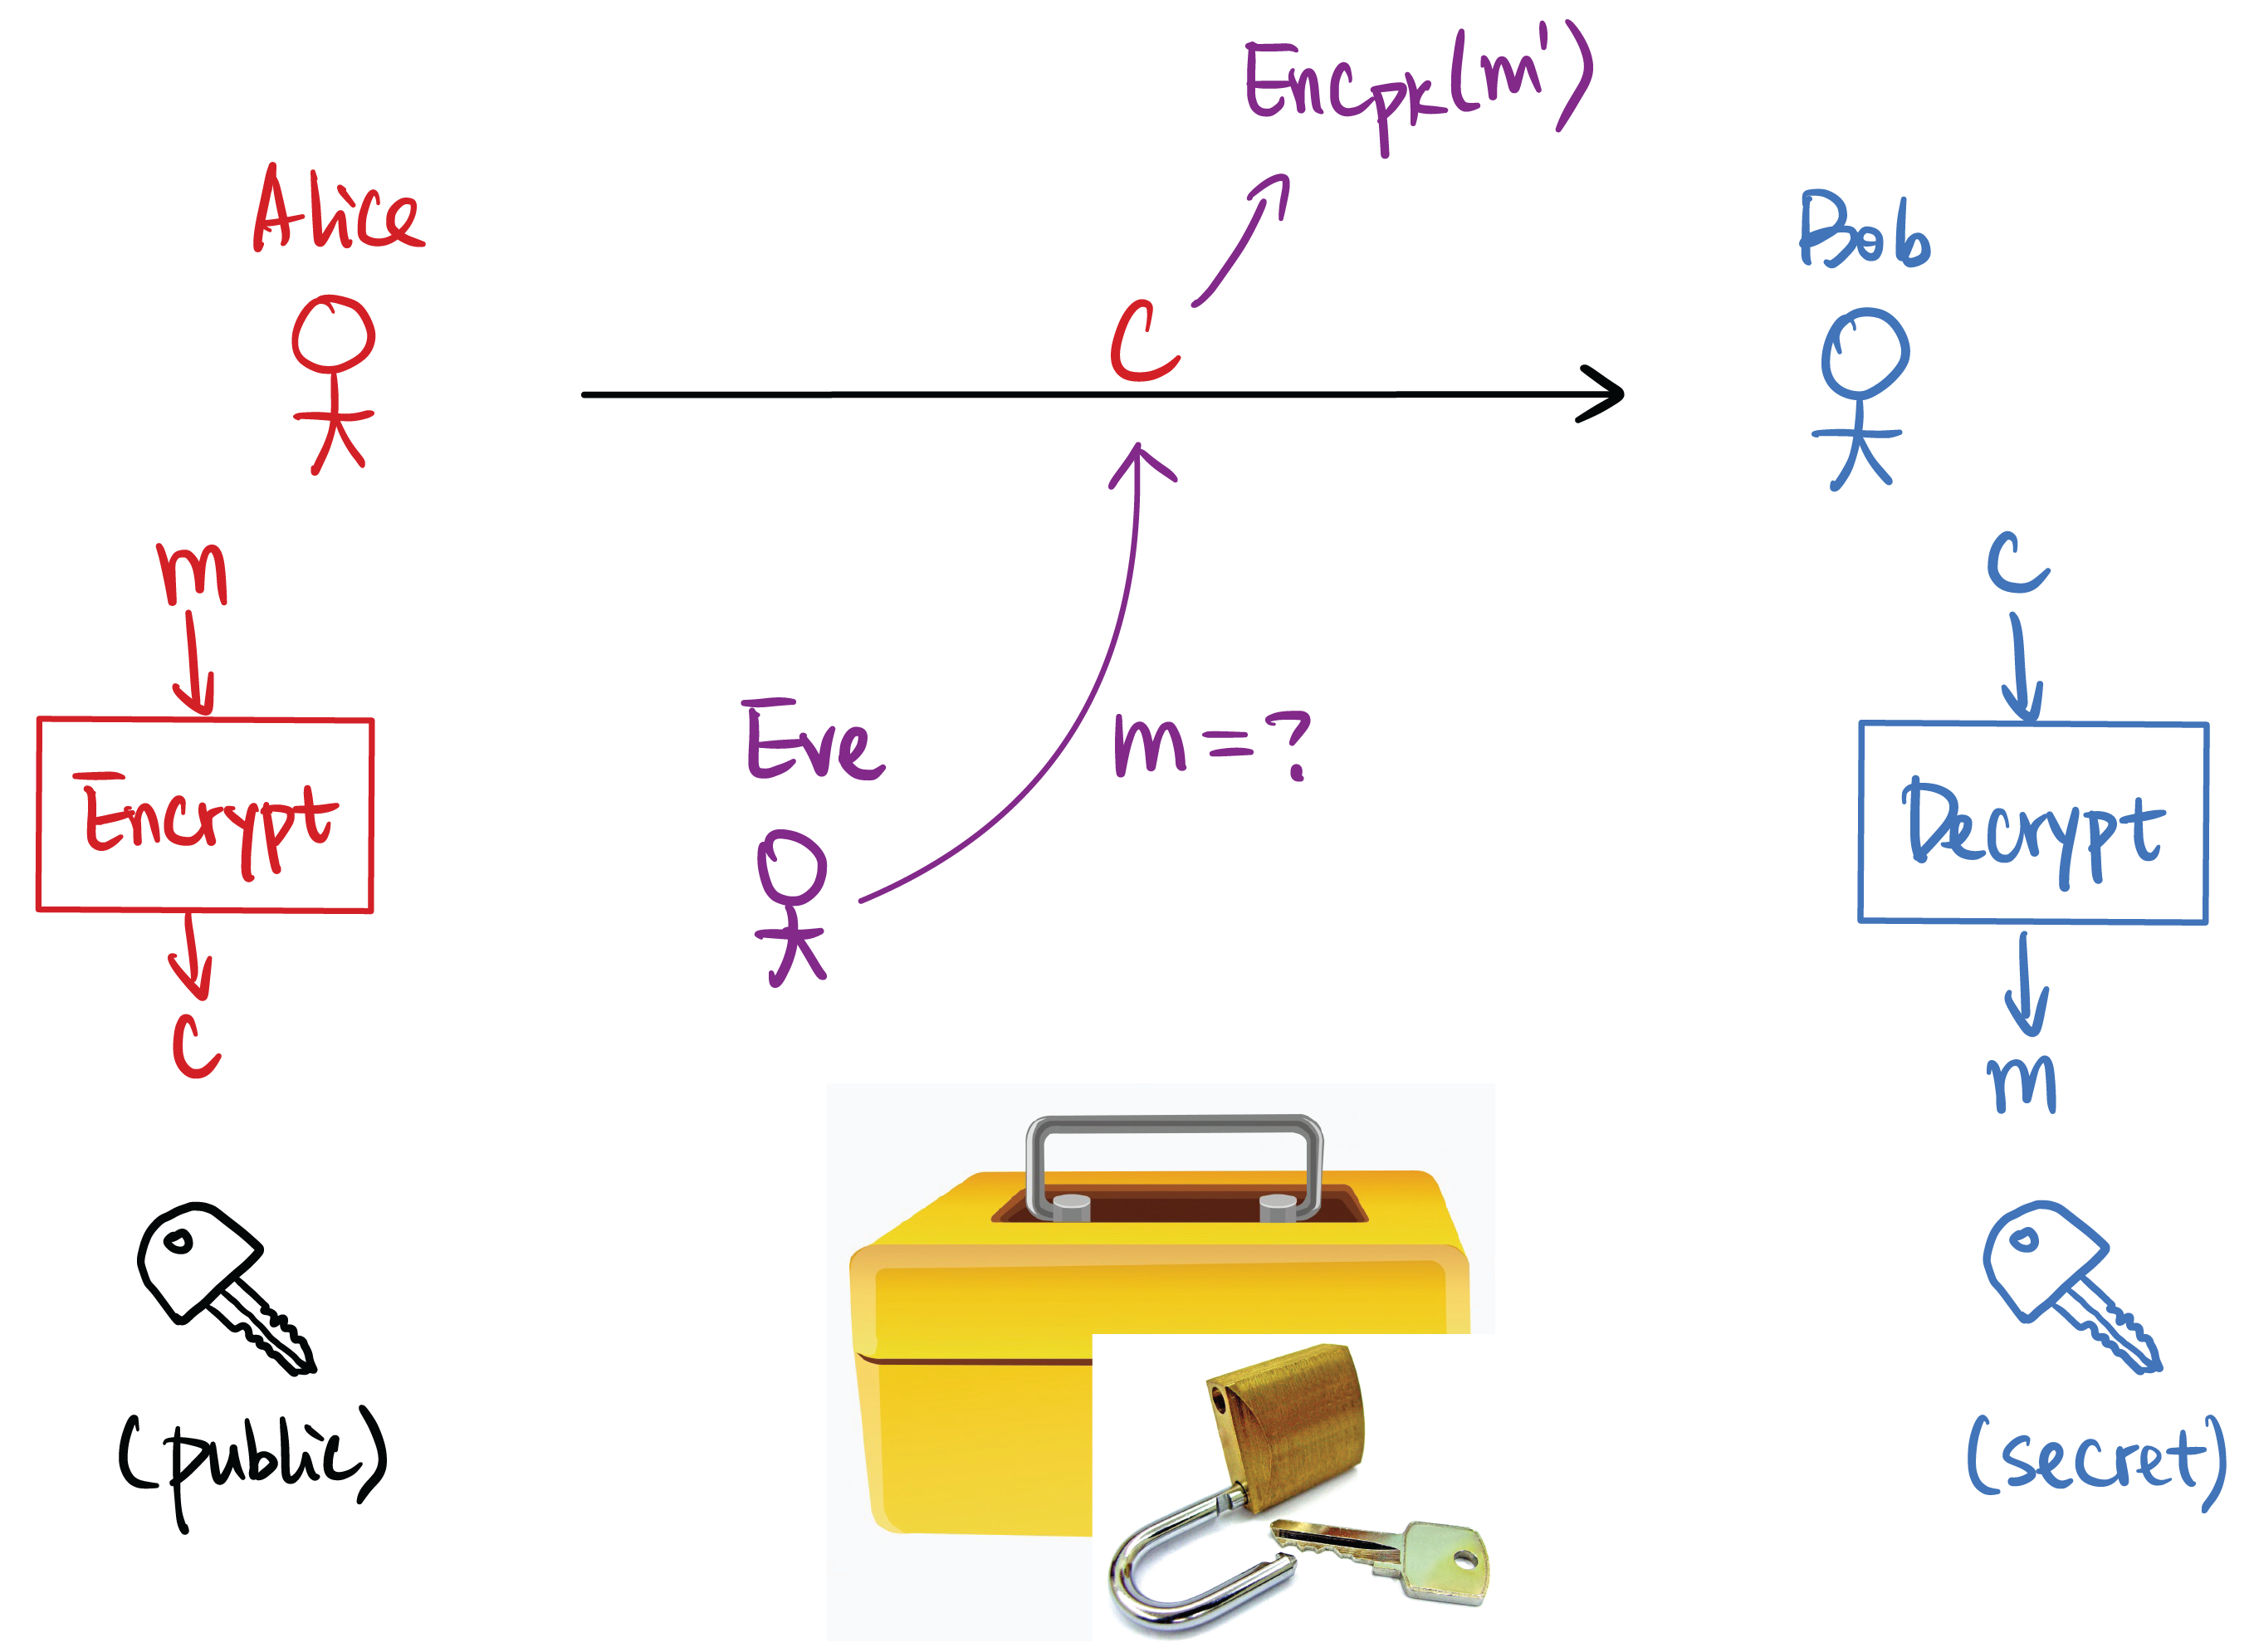
\includegraphics[width=0.9\textwidth]{images/2023-01-26/public_key.png}
    \end{center}

    This is seemingly magic! Bob could publish a public key on his homepage, anyone can encrypt using a public key but only Bob can decrypt. \emph{Stay tuned, we will see public-key encryption schemes next lecture!}
\end{definition}

\subsubsection{Message Integrity}
Alice wants to send a message to Bob again, but Eve is stronger! Eve can now tamper with the message.

\begin{center}
    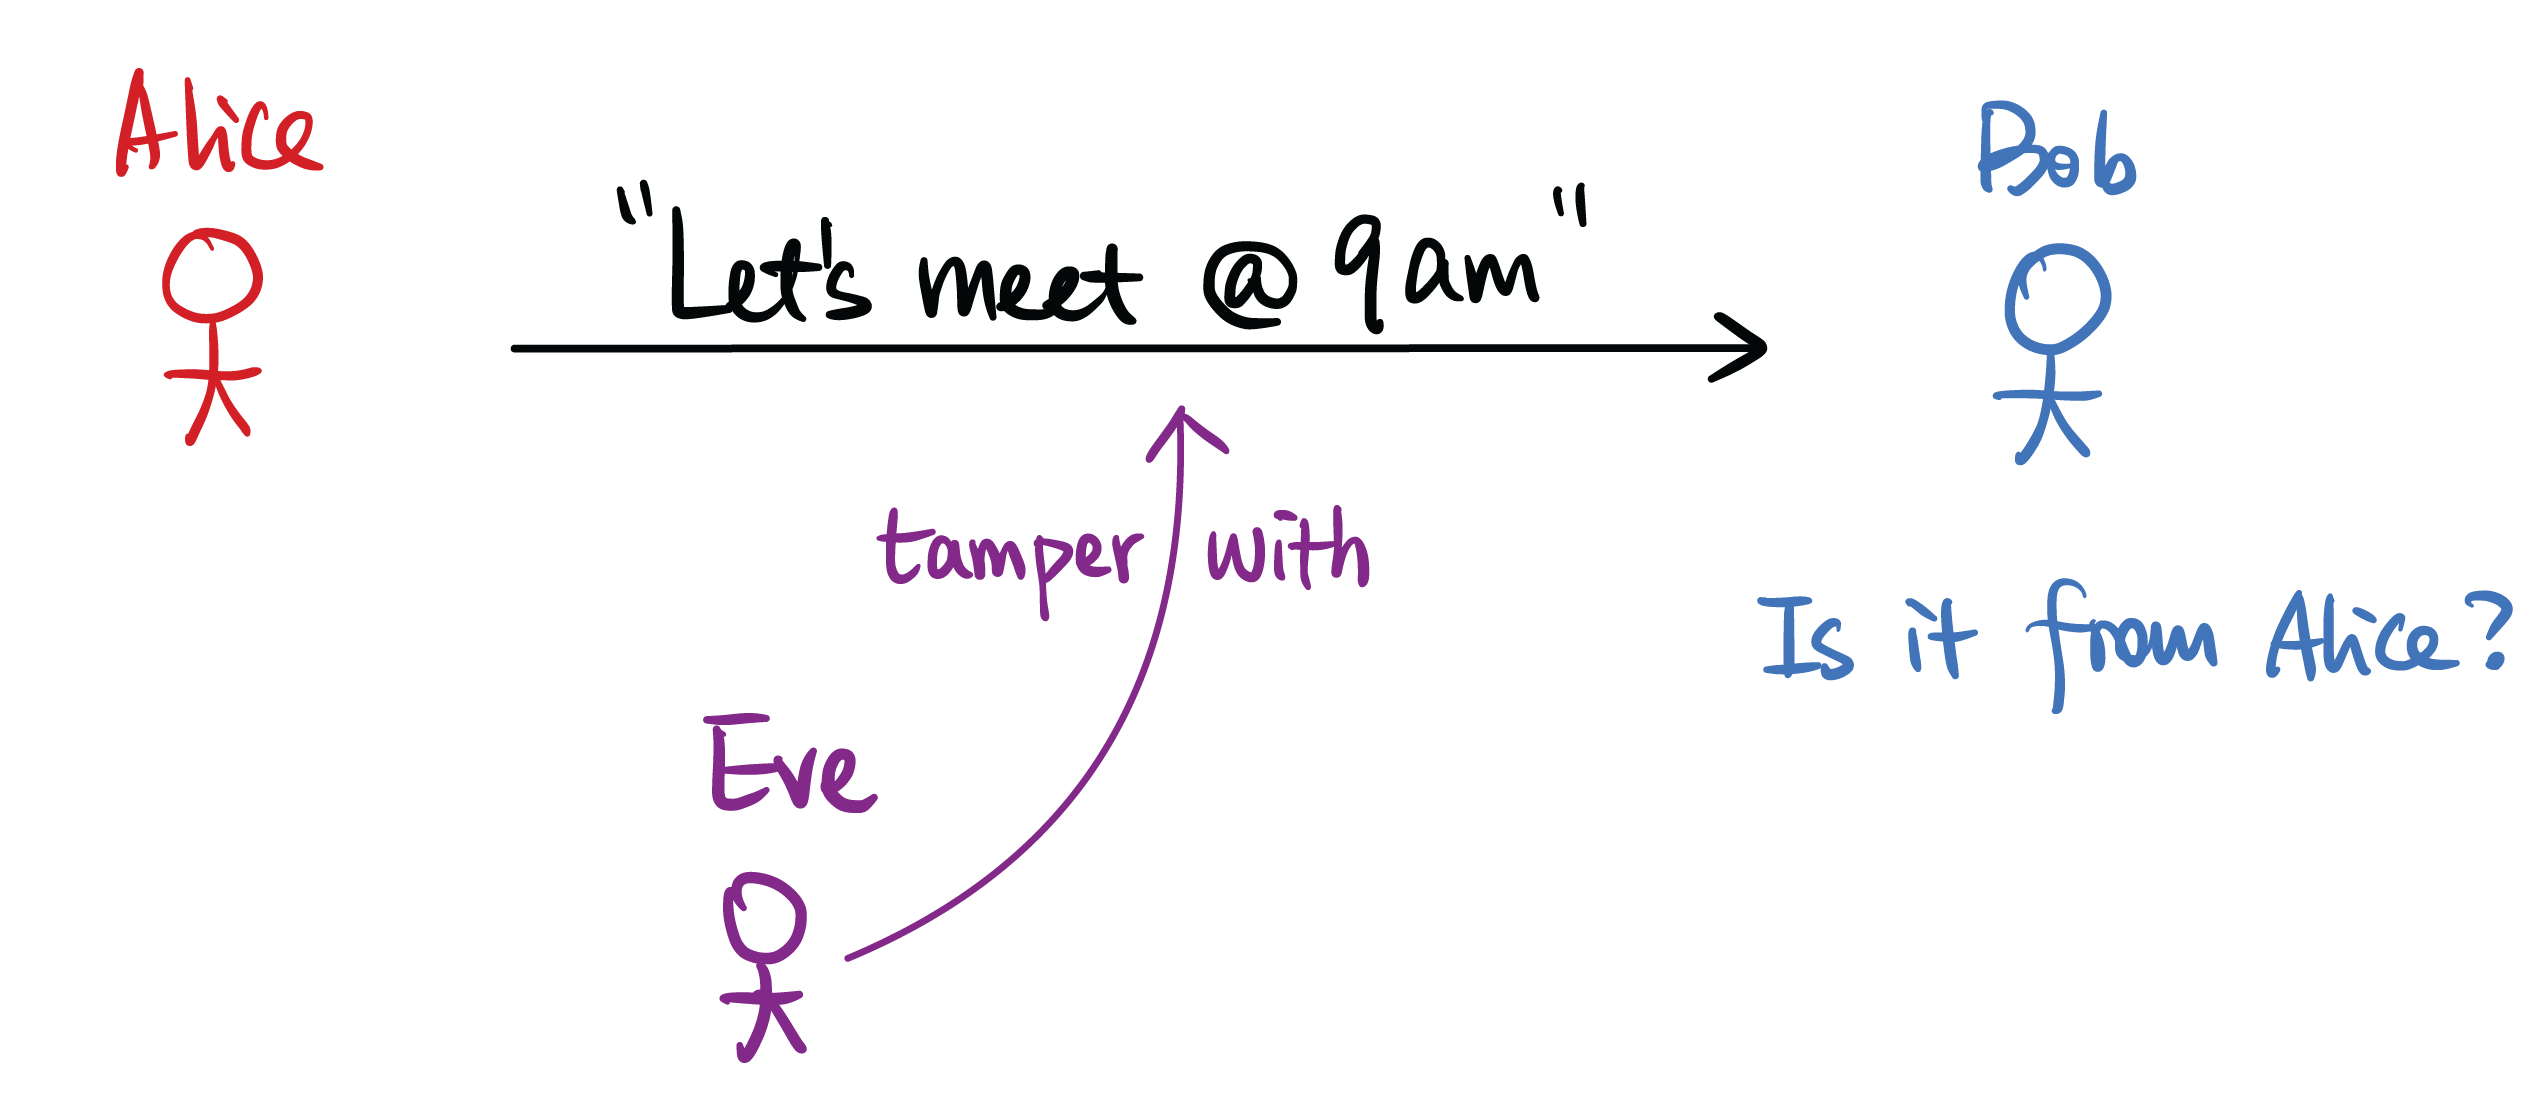
\includegraphics[width=0.9\textwidth]{images/2023-01-26/integrity.png}
\end{center}

Bob wants to ensure that the message \emph{actually} comes from Alice. Does our previous scheme (of encrypting messages) solve this problem? Nope!

Eve can change the ciphertext to something else, they could pretend to be Alice. In secret-key schemes, if Eve figures out the secret-key, they can forge messages from Alice. Even if Eve doesn't know the underlying message, they could still change it to some other ciphertext which might be correlated to the original ciphertext, \emph{without knowing the underlying message}. We'll see how Eve can meaningfully do this in some schemes. Alice could send a message ``Let's meet at $x$ AM'' and Eve could tamper this to say ``Let's meet at $x+1$ AM.''

This is sort of an orthogonal problem to message secrecy. For example, when Alice logs in to Google, Google needs to verify that Alice actually is who she claims to be.

\begin{center}
    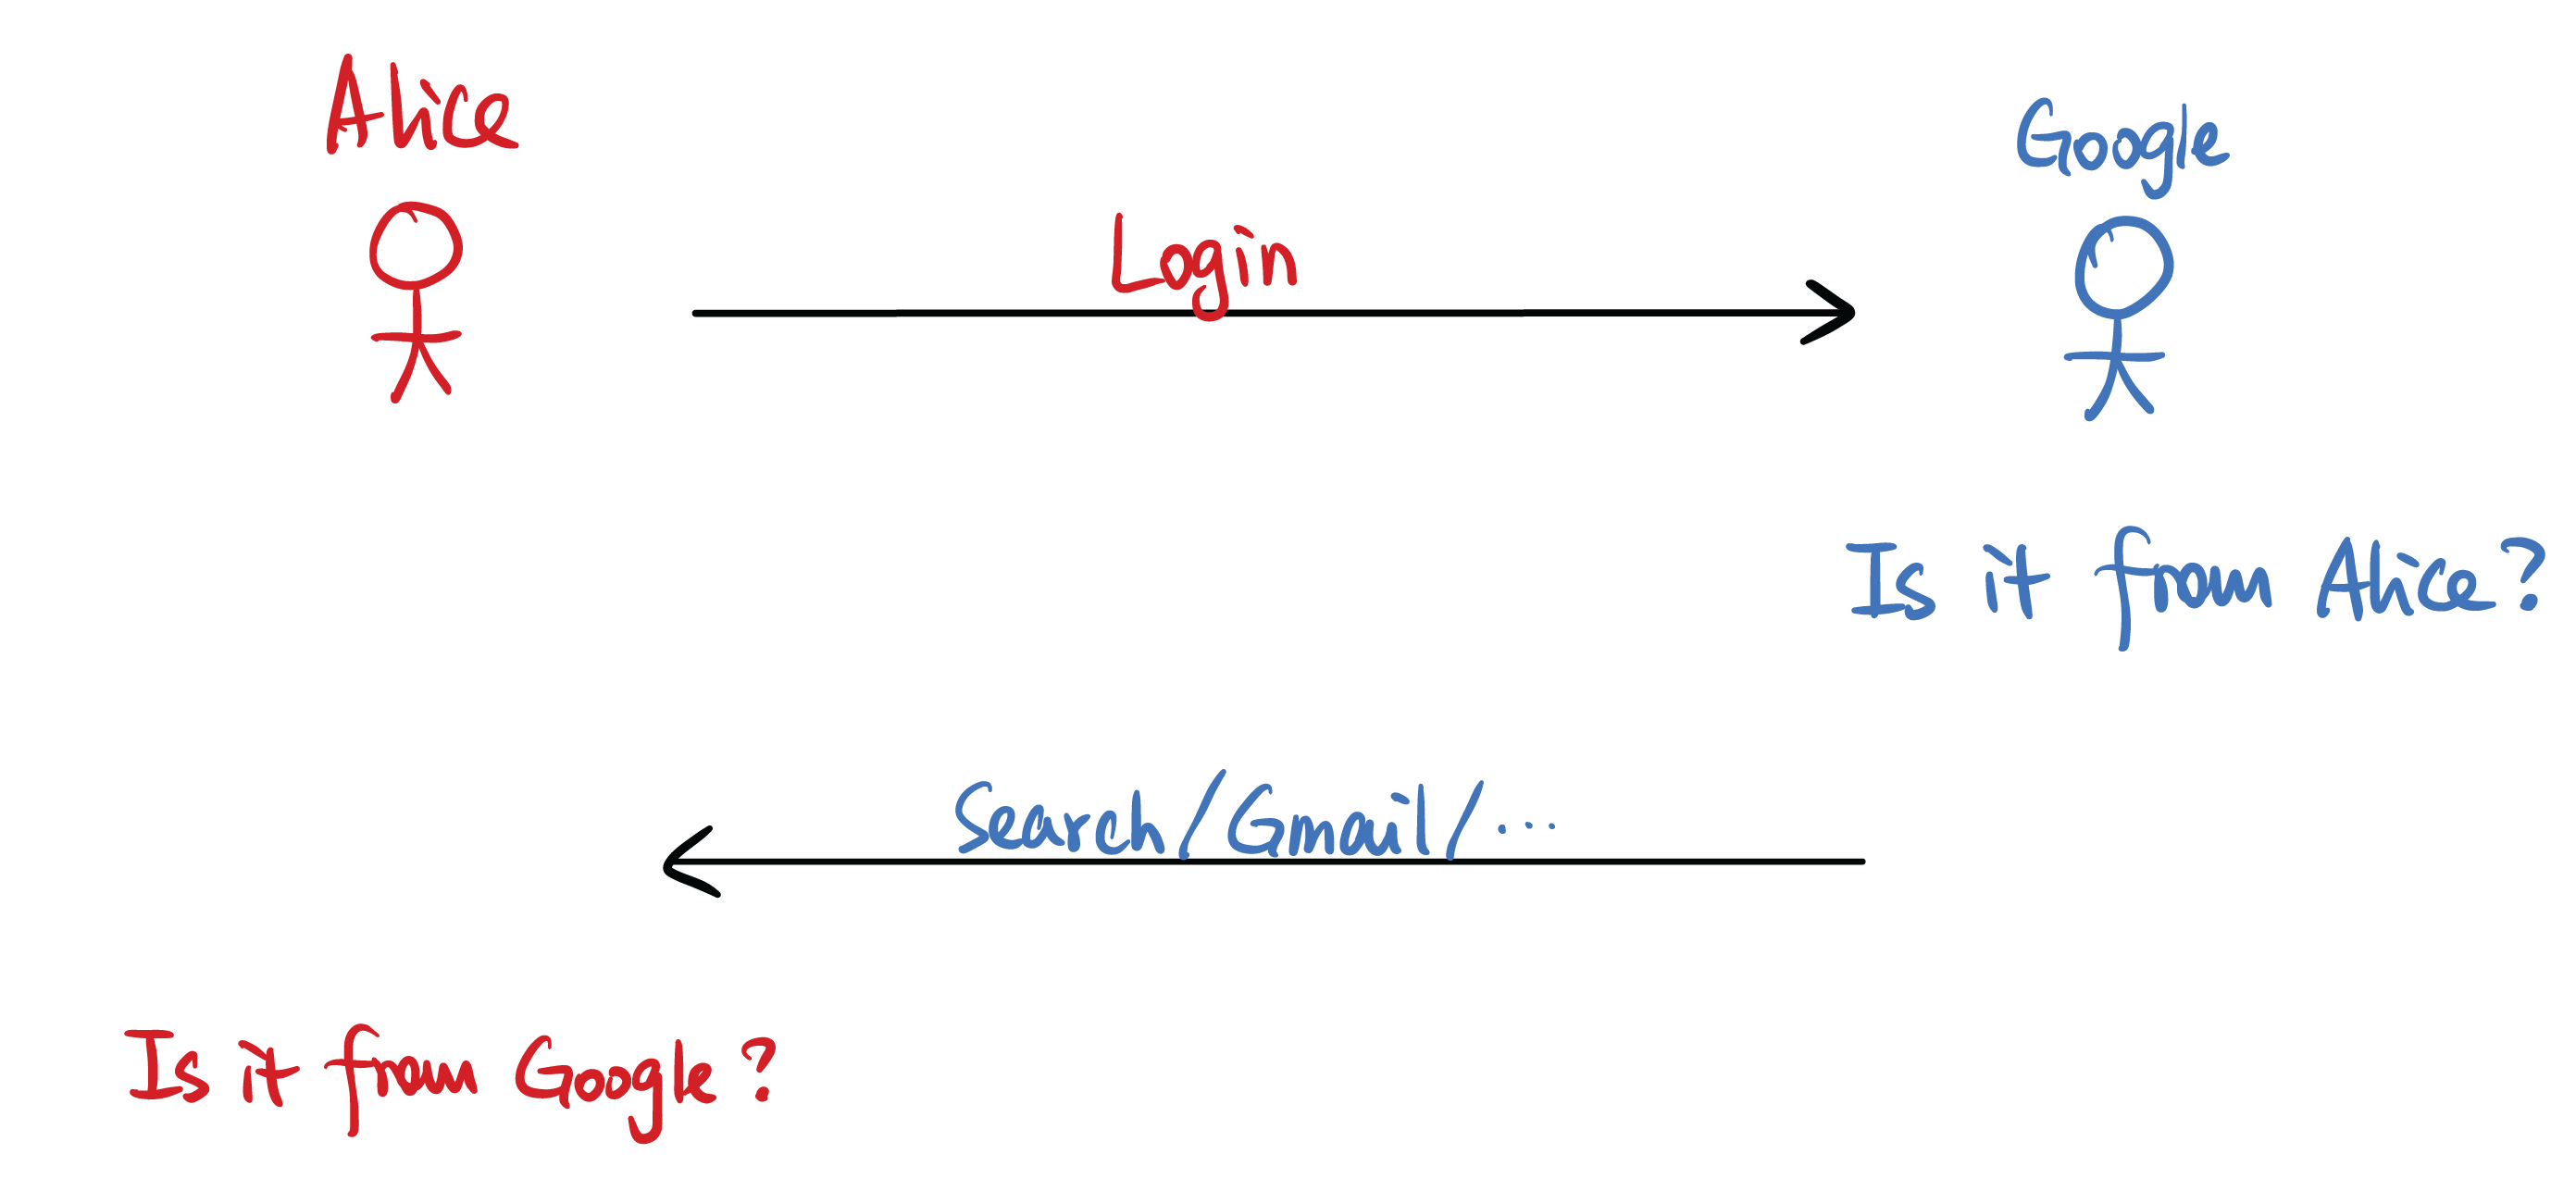
\includegraphics[width=0.9\textwidth]{images/2023-01-26/authentication.png}
\end{center}

\subsection{Project Overview}
\begin{enumerate}
    \setcounter{enumi}{-1}
    \item Warm-up, you will implement some basic cryptographic schemes.
    \item Secure Communication: what was just introduced.
    \item Secure Authentication: how to authenticate yourself to a server, also mentioned just now.
    \item Zero-Knowledge Proofs: we'll use ZKPs to implement a secure voting scheme.
    \item Secure Multiparty Computation: we'll implement a way to run any function securely between two parties.
    \item Fully Homomorphic Encryption: a form of post-quantum cryptography.
\end{enumerate}
We'll quickly introduce the concepts used in the projects.

\subsubsection{Zero-Knowledge Proofs}
This is to prove something without \emph{revealing} any additional knowledge.
\begin{example*}
    Alice claims to be able to differentiate between Coca-Cola and Pepsi! She wants to prove this to Bob without revealing her secrets.

    Bob will randomly sample a bit $b\overset{\$}{\leftarrow}\{0, 1\}$, with $b=0$ being Coca-Cola and $b=1$ being Pepsi. Bob will let Alice taste this drink. Alice will give a guess $b'$ of what drink it is.

    \begin{center}
        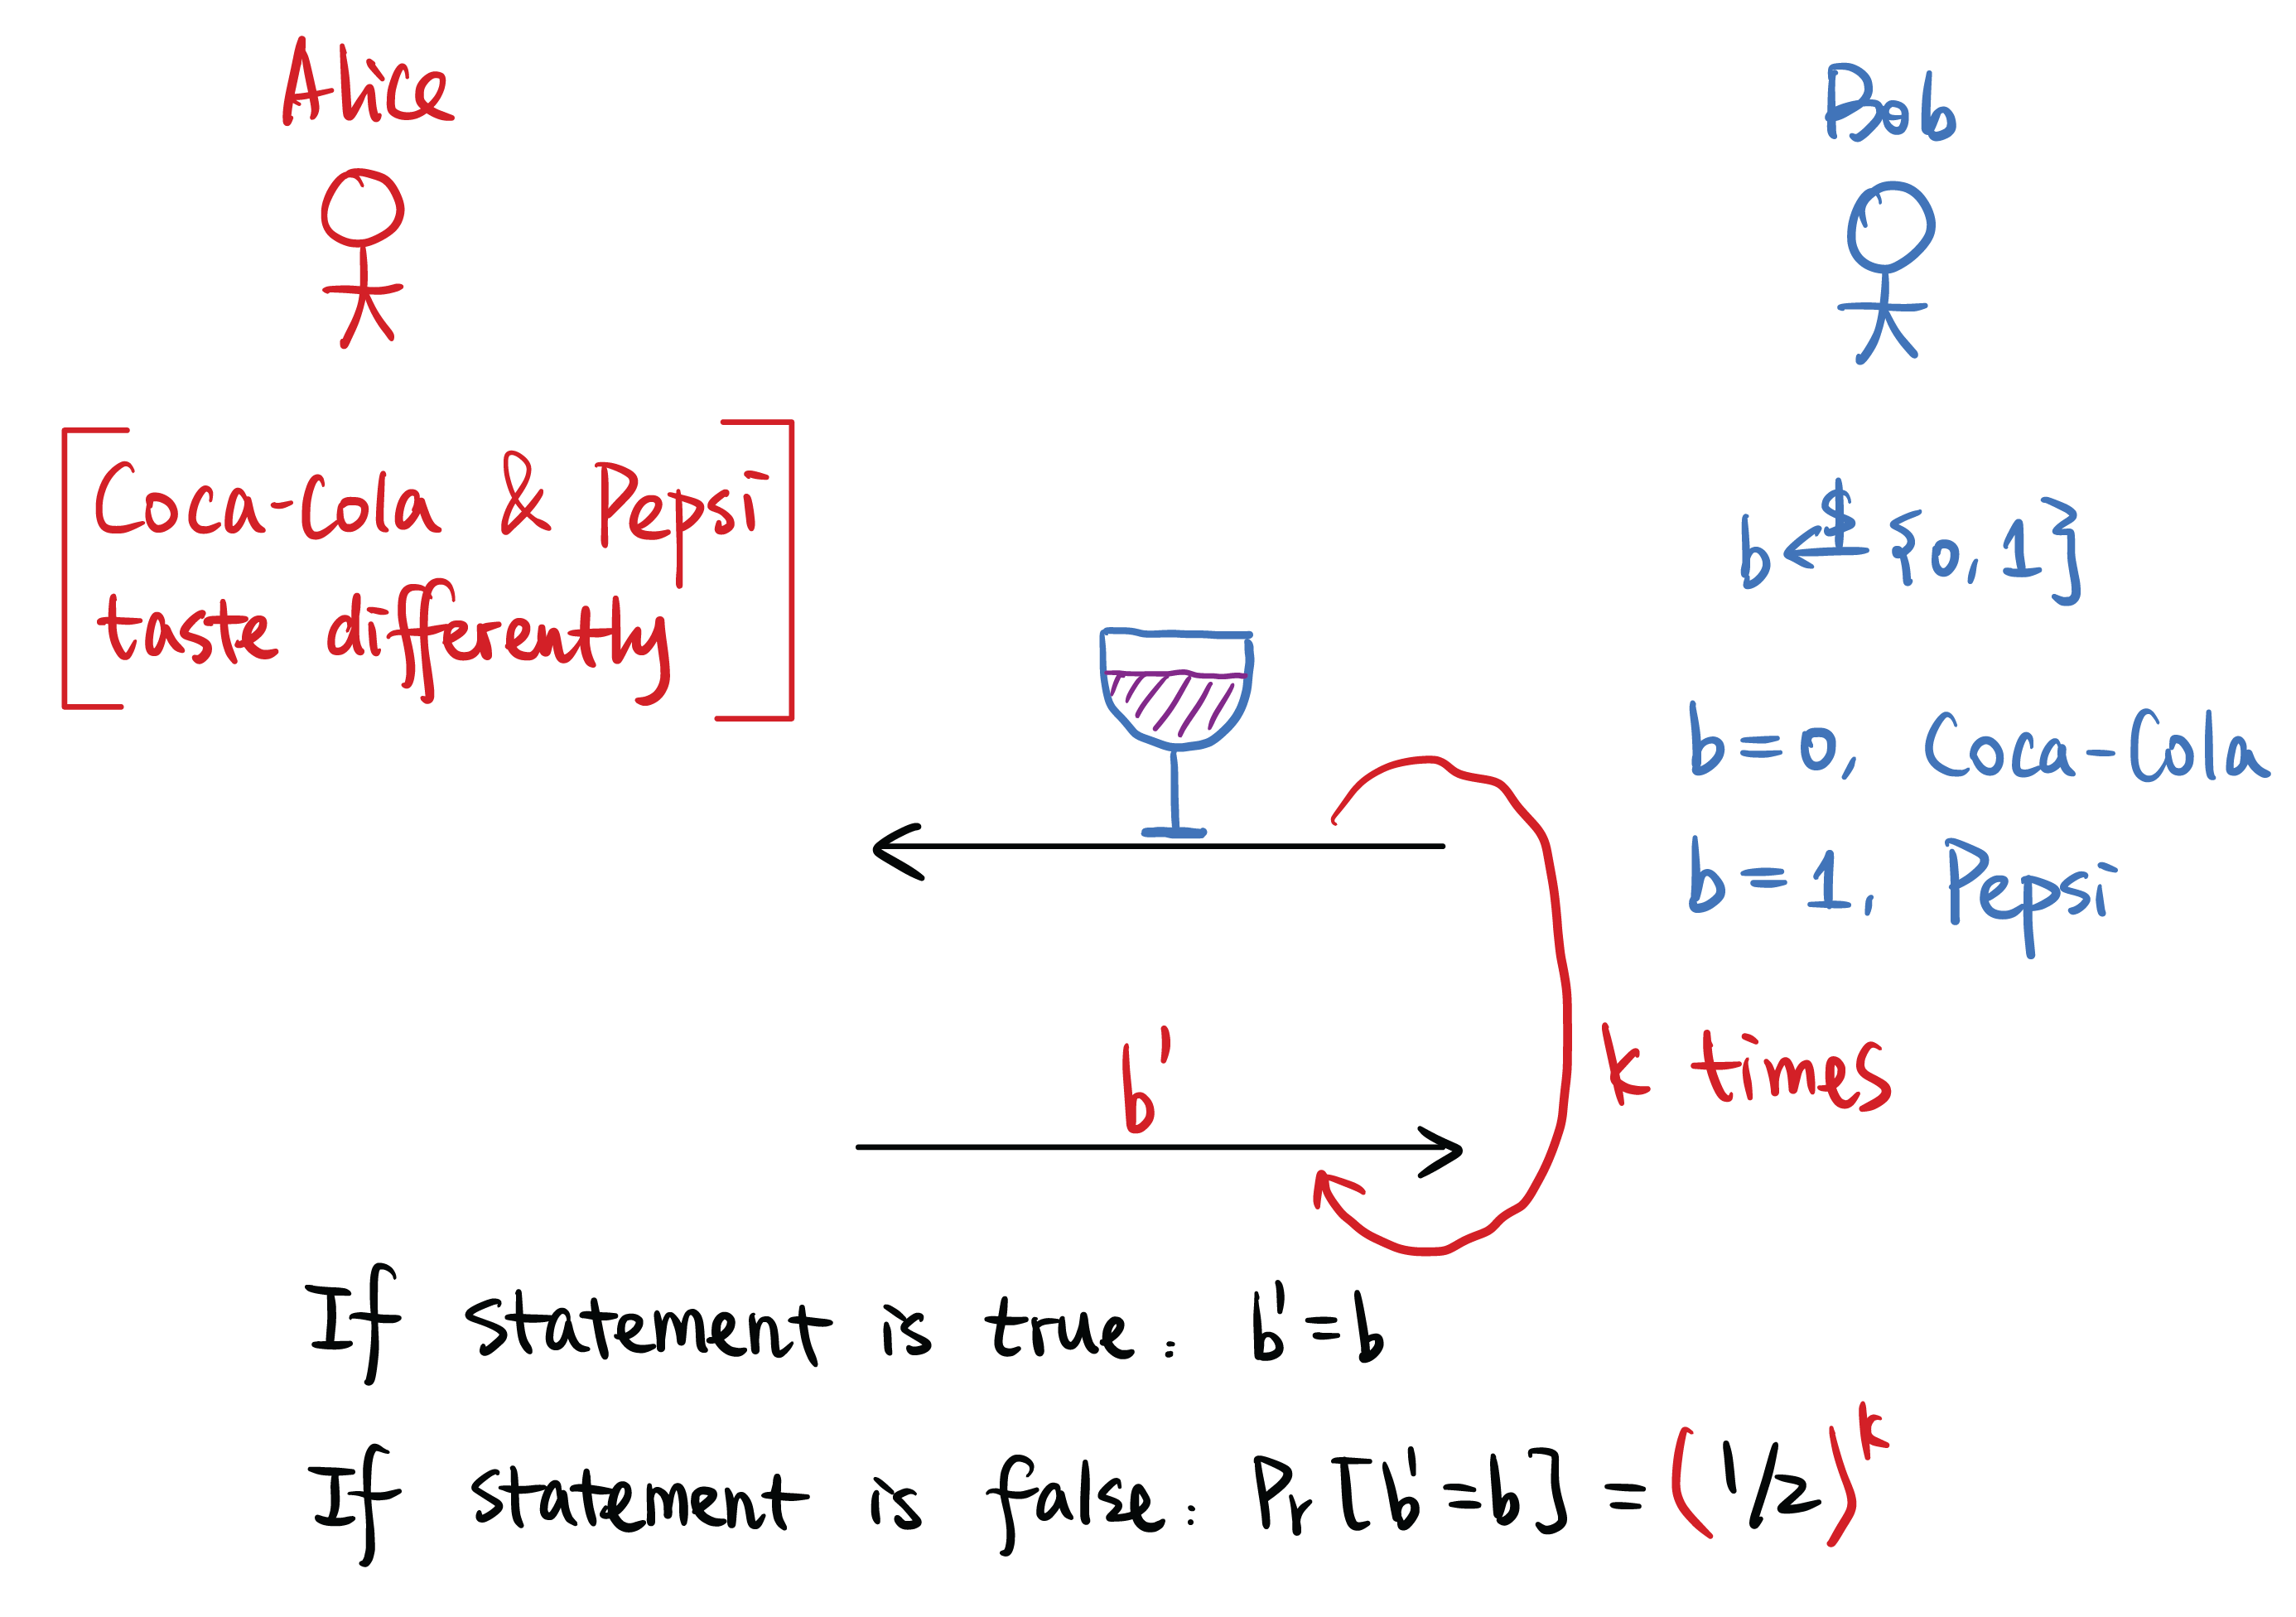
\includegraphics[width=0.9\textwidth]{images/2023-01-26/zk_cola.png}
    \end{center}

    If the statement is true, $b' = b$ (Alice gives the correct prediction).

    If the statement is false, $\Pr[b' = b] = \frac{1}{2}$ (Alice is guessing at $0.5$ probability).

    To enhance this, we can run this a total of $k$ times. If we run it enough times, Bob will be more and more confident in believing this. Alice getting this correct by chance has a $\frac{1}{2^k}$ probability.

    The key idea, however, is that Bob doesn't gain any knowledge of how Alice differentiates.

    \begin{remark*}
        This is a similar strategy in proving graph non-isomorphism.

        For people who have seen this before, generally speaking, any $\textsf{NP}$ language can be proved in zero-knowledge. Alice has the \emph{witness} to the membership in $\textsf{NP}$ language.
    \end{remark*}
\end{example*}

\subsubsection{Secure Multi-Party Computation}
\begin{center}
    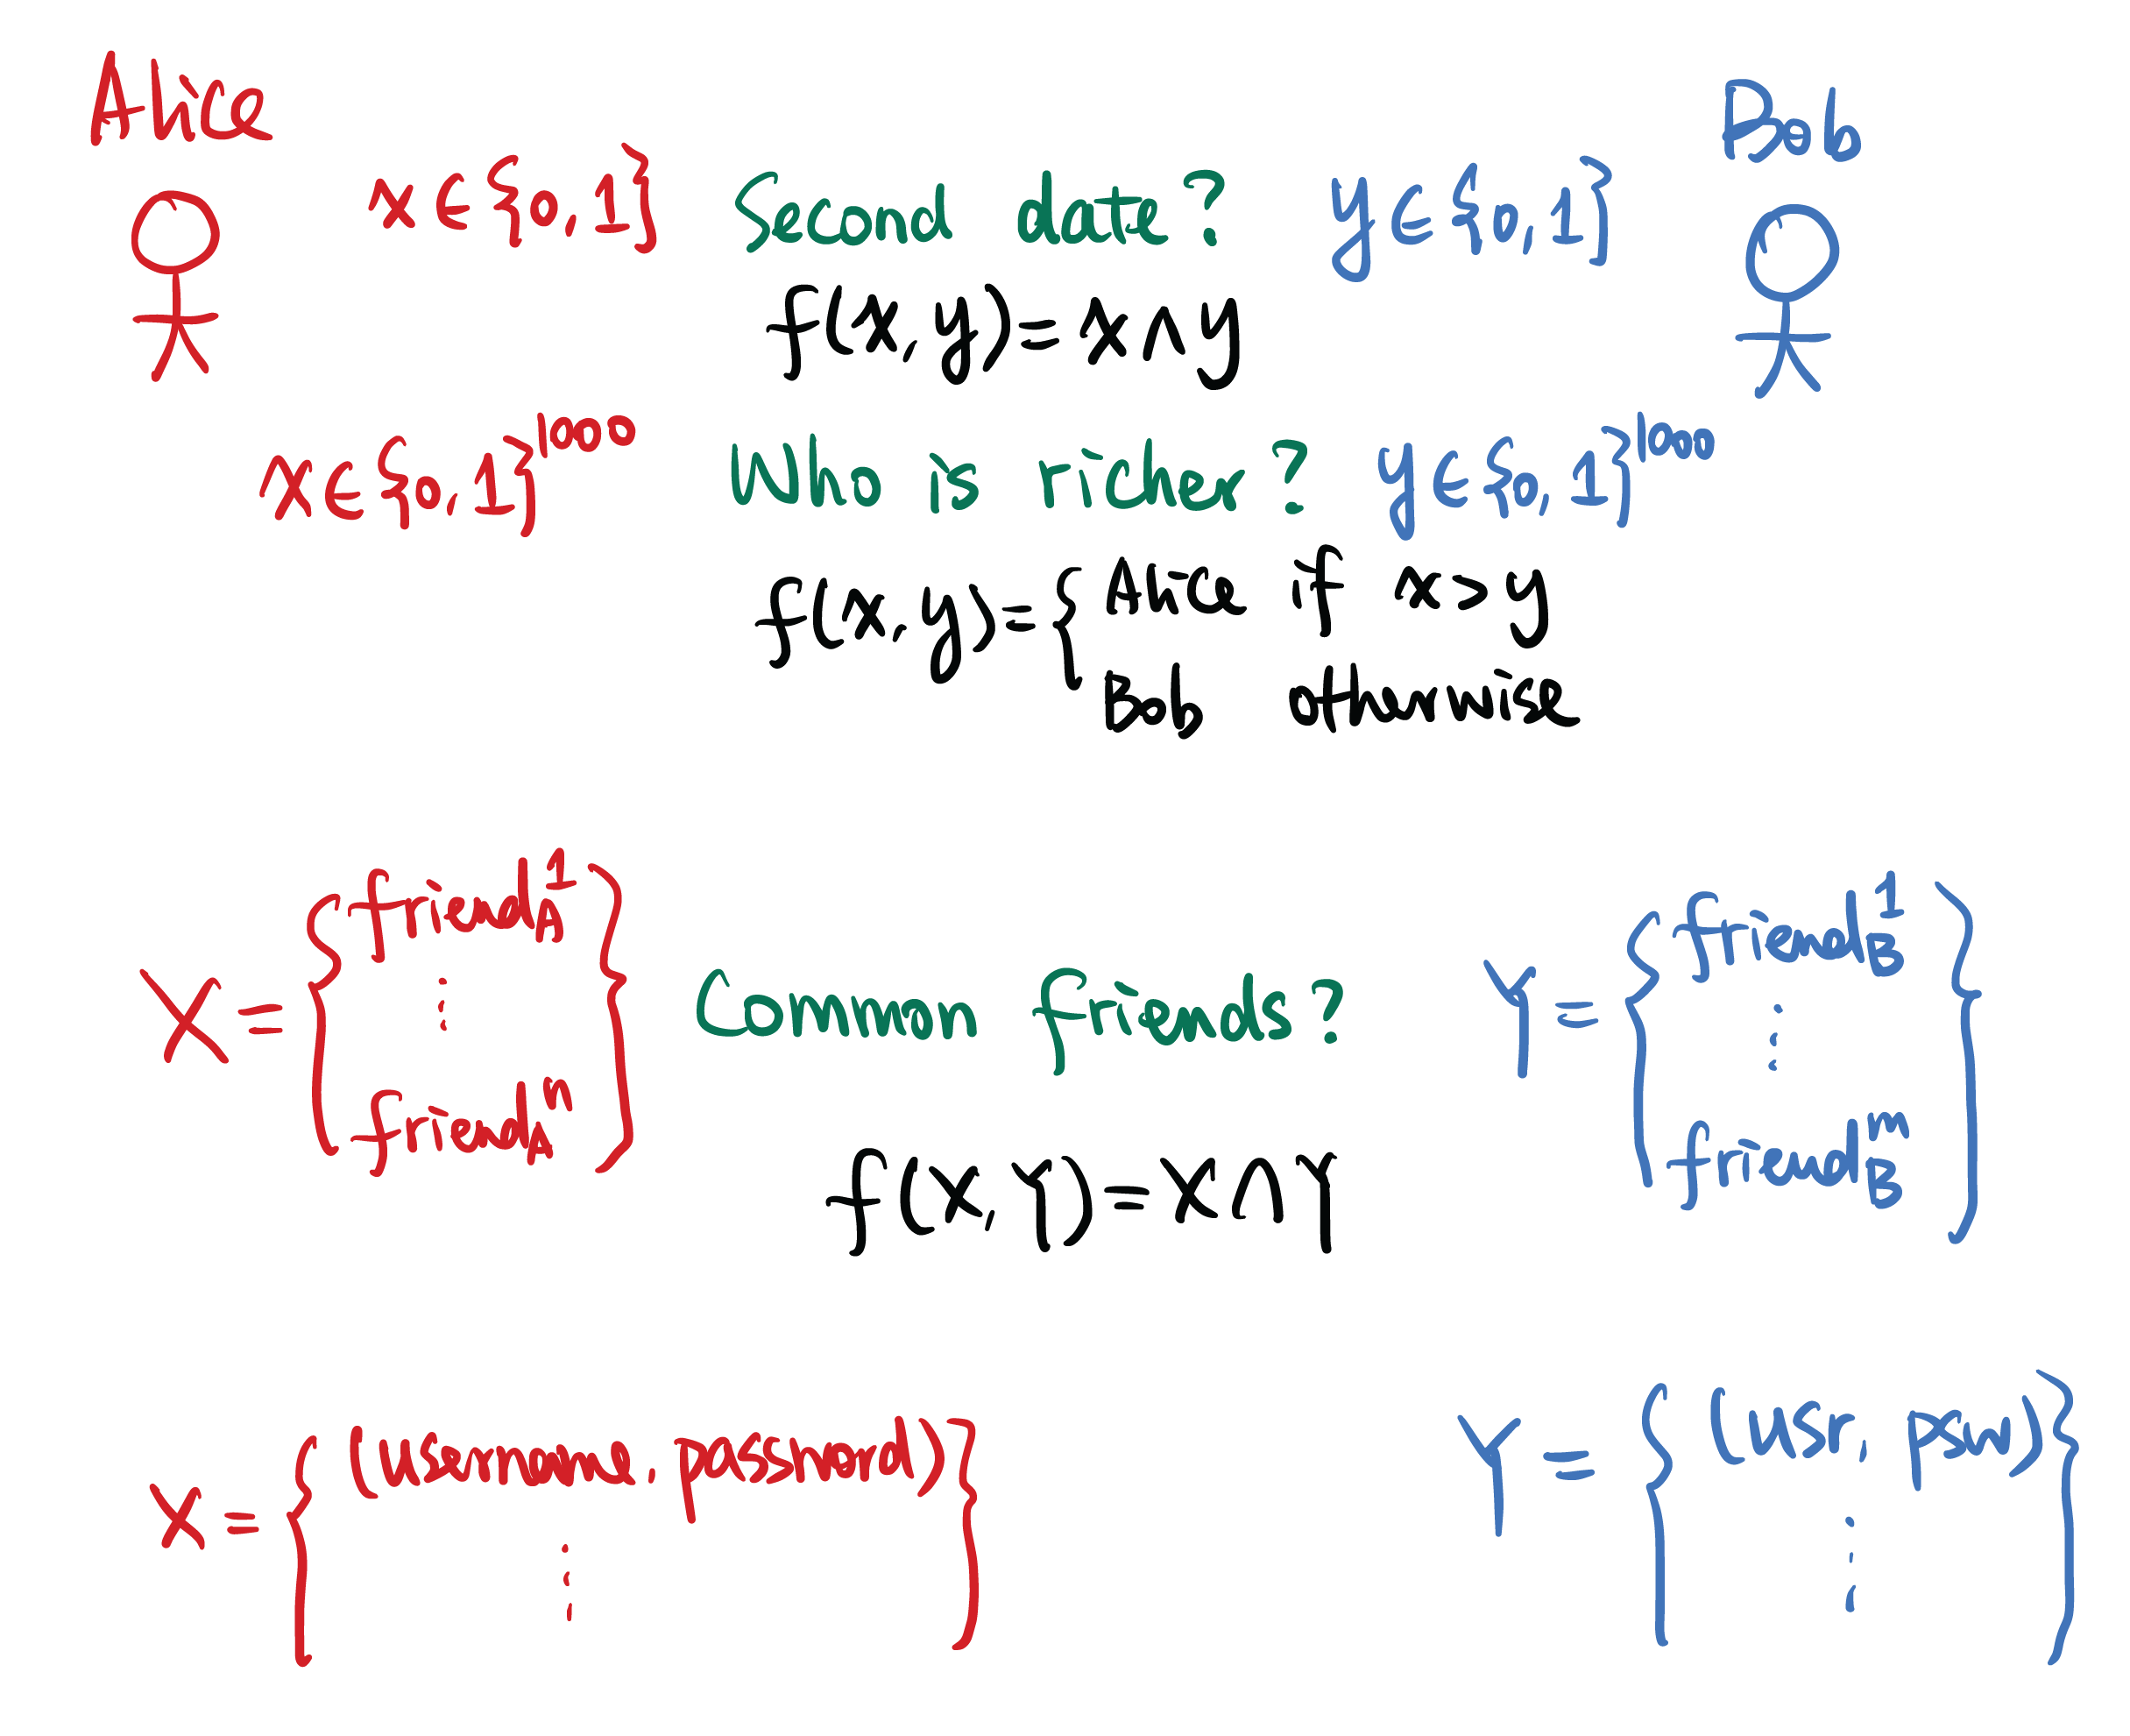
\includegraphics[width=0.9\textwidth]{images/2023-01-26/secure_mpc.png}
\end{center}

\begin{example*}[Secure \textsf{AND}]
    Alice and Bob go on a first date, and they want to figure out whether they want to go on a second date. They will only go on a second date if and only if both agree to a second date.

    How will they agree on this? They could tell each other, but this could be embarrassing. One way is for them to share with a third-party (this is what dating apps do!). However, there might not always be an appropriate third party (in healthcare examples, not everyone can be trusted with the data).

    In this case, Alice has a choice bit $x\in\{0, 1\}$ and Bob has a choice bit $y\in\{0, 1\}$. They are trying to jointly compute $f(x, y) = x\land y$.
\end{example*}

\begin{example*}[Yao's Millionaires' Problem]
    Perhaps, Alice and Bob wants to figure out who is richer. The inputs are $x\in\{0, 1\}^{1000}$ and $y\in\{0, 1\}^{1000}$ (for simplification, let's say they can express their wealth in 1000 bits). The output is the person who has the max.
    \[f(x, y) = \begin{cases}
            \text{Alice} & \text{if }x > y  \\
            \text{Bob}   & \text{otherwise}
        \end{cases}\]
\end{example*}

\begin{example*}[Private Set Intersection]\label{ex:psi}
    Alice and Bob meet for the first time and want to determine which of their friends they share. However, they do not want to reveal who specifically are their friends.

    $X$ is a set of A's friends $X = \{\mathsf{friend}_A^1, \mathsf{friend}_A^2, \cdots, \mathsf{friend}_A^n\}$ and Bob also has a set $Y = \{\mathsf{friend}_B^1, \mathsf{friend}_B^2, \cdots, \mathsf{friend}_B^m\}$. They want to jointly compute \[f(X, Y) = X\cap Y.\]

    You might need to reveal the cardinality of these sets, but you could also pad them up to a maximum number of friends.

    This has a lot of applications in practice! In Google Chrome, your browser will notify you that your password has been leaked on the internet, without having access to your passwords in the clear. $X$ will be a set of \emph{your} passwords, and Google will have a set $Y$ of \emph{leaked} passwords. The \emph{intersection} of these sets are which passwords have been leaked over the internet, without revealing all passwords in the clear.
\end{example*}
\begin{ques*}
    Isn't the assumption that the size is revealed weaker than using a trusted third-party?

    Yes, however in some cases (hospital health records), parties are legally obliged to keep data secure. We wish for security more than the secrecy of cardinality.
\end{ques*}

In the general case, Alice and Bob have some inputs $x$ and $y$ with bounded length, and they want to jointly compute some function $f$ on these inputs. This is \ul{Secure Two-Party Computation}. Furthermore, there could be multiple parties $x_1, \dots, x_n$ that jointly compute $f(x_1, \dots, x_n)$ that hides each input. This is \ul{Secure Multiparty Computation}.

We'll explore a toy example with the bit-\textsf{AND} from the dating example.

\begin{example*}[Private Dating]
    Alice and Bob have choice bits $x\in\{0, 1\}$ and $y\in\{0, 1\}$ respectively. There is a \emph{physical} round table with $5$ identical slots, one already filled in with a $1$ facing down.

    \begin{center}
        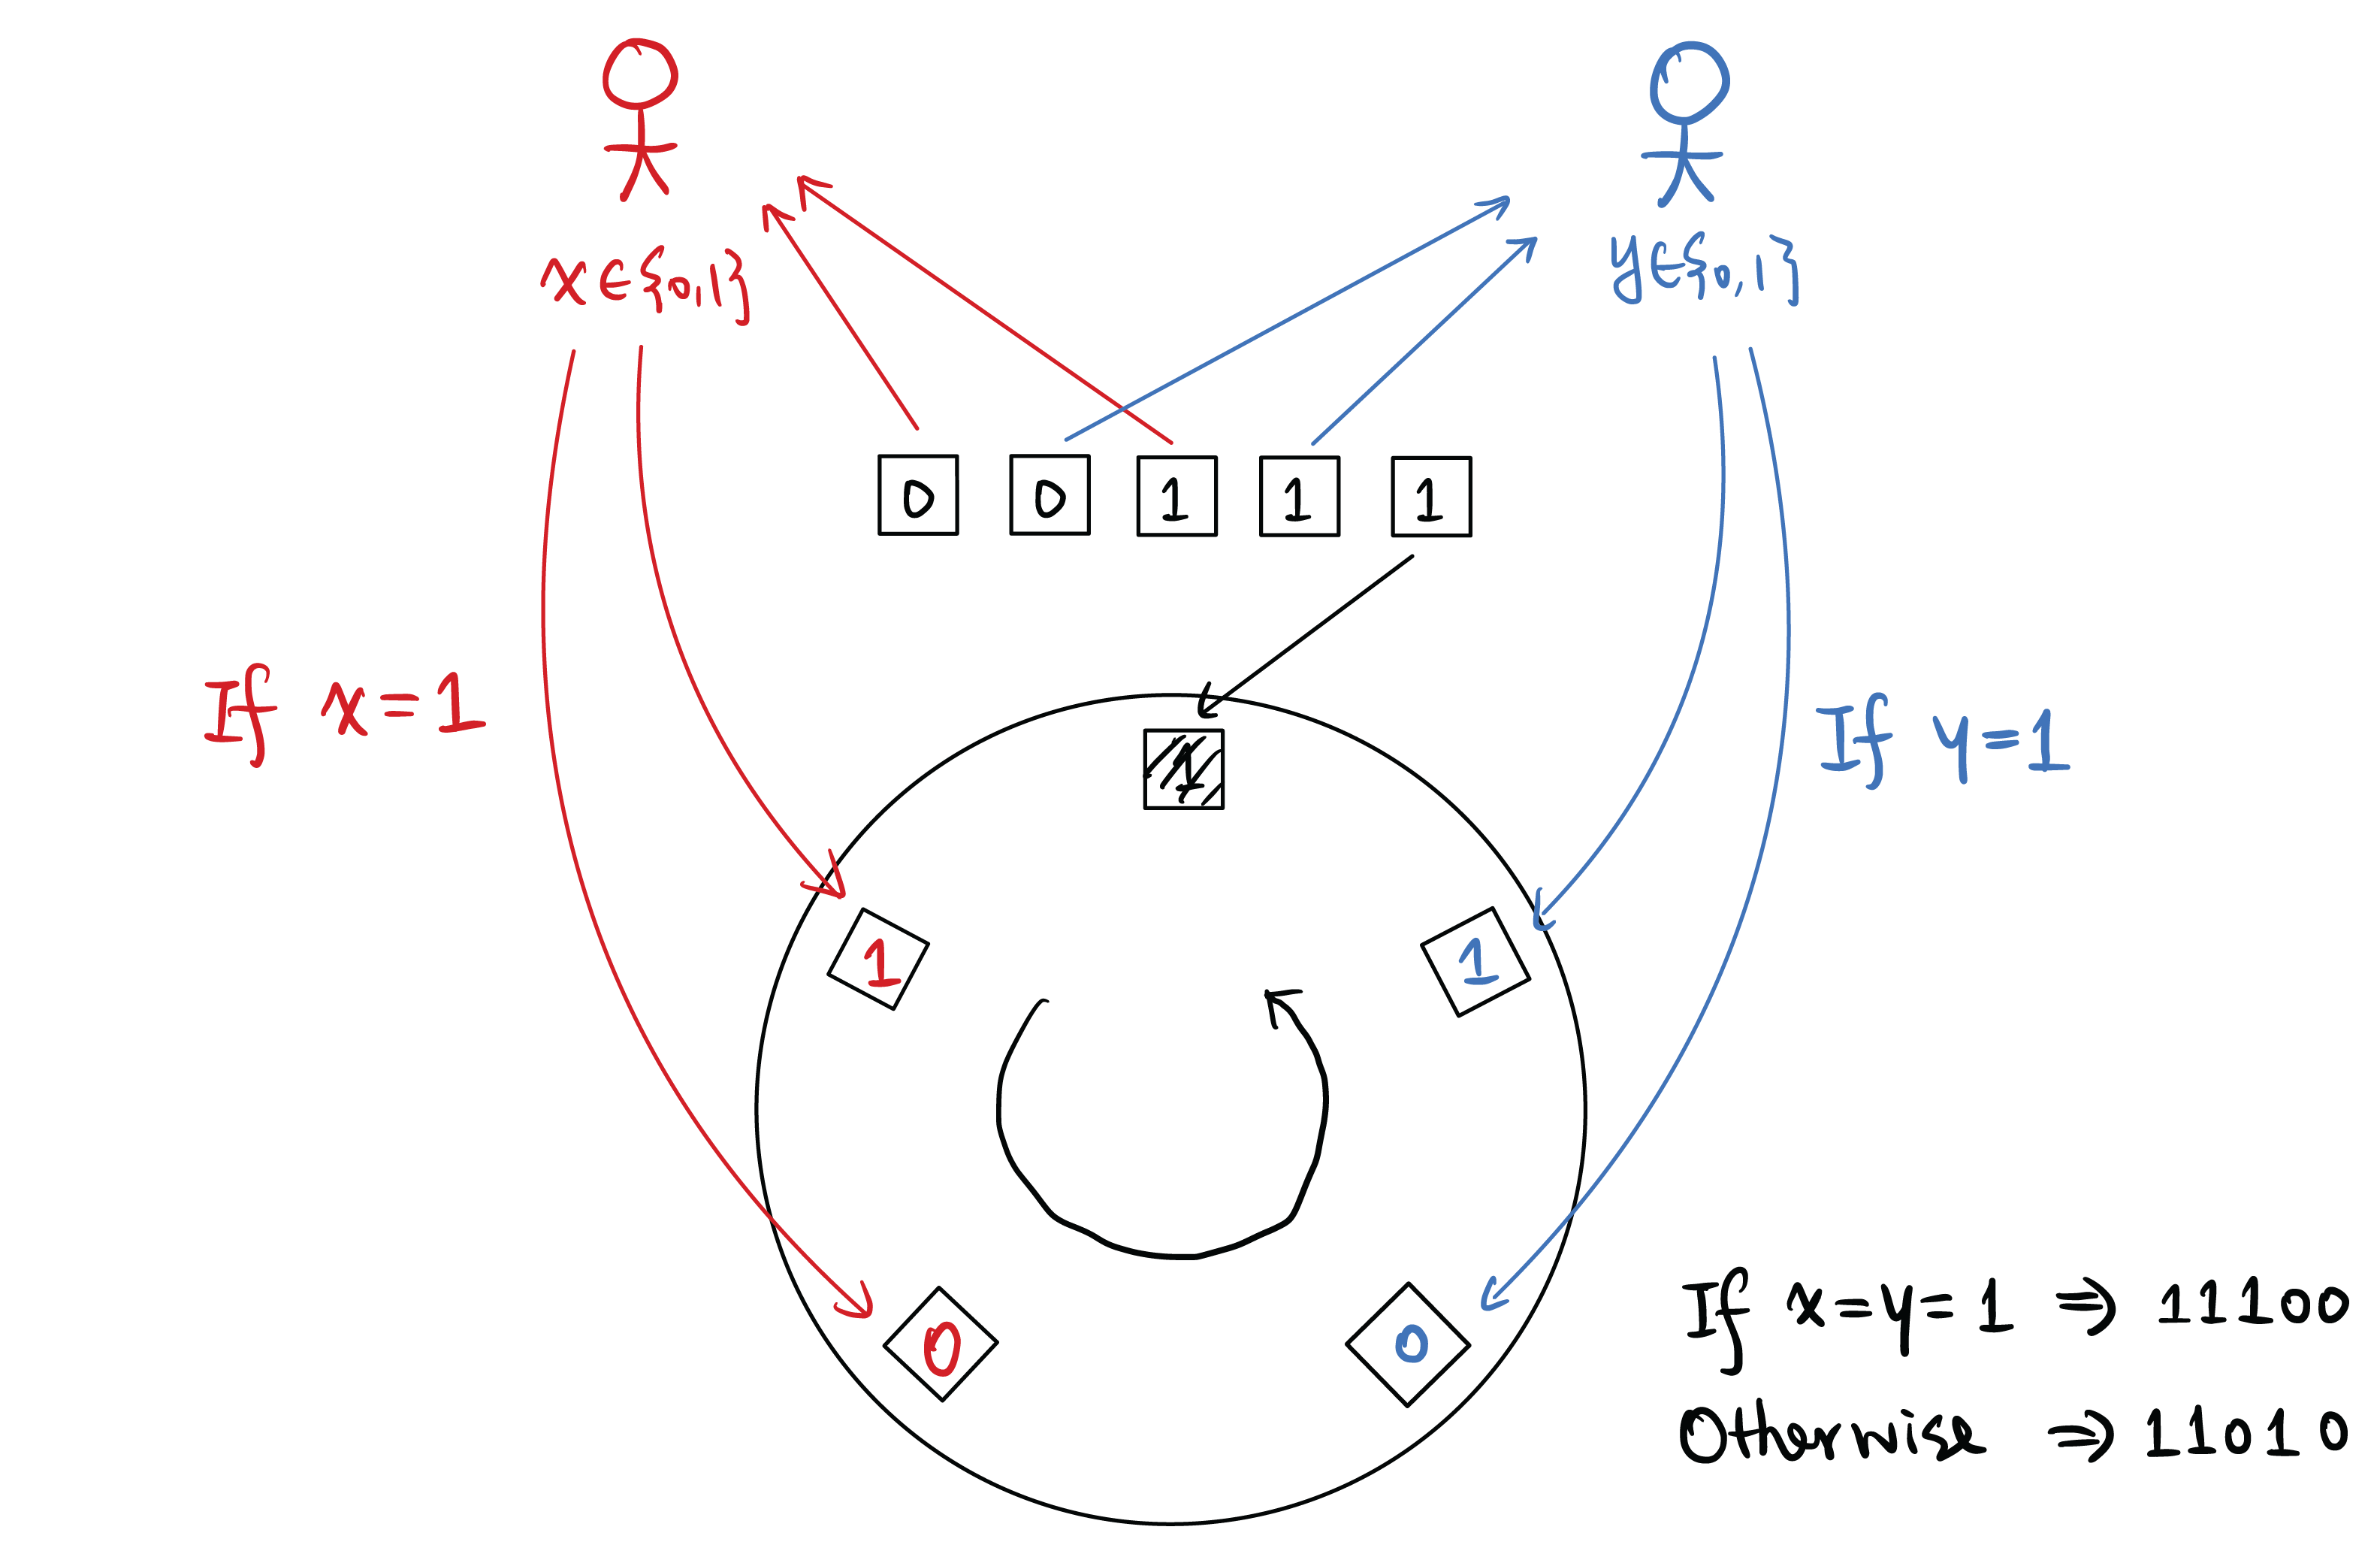
\includegraphics[width=0.9\textwidth]{images/2023-01-26/private_dating.png}
    \end{center}

    Alice and Bob each have identical $0, 1$ cards (each of the $0$ and $1$ cards are indistinguishable from cards of the same value). Alice places her cards on the 2 slots in some order, and Bob does the same.

    They then spin the table around and reveal all the cards, learning $x\land y$.

    If $x = 1$, Alice places it as $1$ on top of $0$, and if $y = 1$, Bob places it as $1$ on top of $0$ as well. Otherwise, they flip them. If $x = y = 1$, then the $0$'s will be adjacent. If $x \neq y$, the order will be $1,1,0,1,0$ (the $0$'s are not adjacent), regardless of which of Alice or Bob produced $x = 0$ (or both!).
\end{example*}
\begin{ques*}
    If Alice puts $1$, and the output is $0$, she could infer the information from Bob. However, this is allowed. Whatever can be inferred from the desired output is inferred.

    The more sensitive part is when if you put a $0$, you don't learn whether the other party also put down a $0$.
\end{ques*}
\emph{This is a toy example! It doesn't use cryptography at all! Two parties have to sit in front of a table. This is called card-based cryptography. We will be using more secure primitives.}

\subsubsection{Fully Homomorphic Encryption}
We'll come back to the secure messaging example.

Alice wants to send Bob a message. She encrypts it somehow and sends a ciphertext $c_1 = \mathsf{Enc}(m_1)$. A nice feature for some encryption schemes is for Eve to do some computation homomorphically on the ciphertexts. Eve might possibly want to add ciphertexts (that leads to plaintext adding)
\[c_1 = \mathsf{Enc}(m_1), c_2 = \mathsf{Enc}(m_2)\Rightarrow c' = \mathsf{Enc}(m_1 + m_2)\]
or perhaps $c'' = \mathsf{Enc}(m_1\cdot m_2)$, or compute arbitrary functions. \emph{Sometimes}, this is simply adding $c_1 + c_2$, but usually not.

\begin{center}
    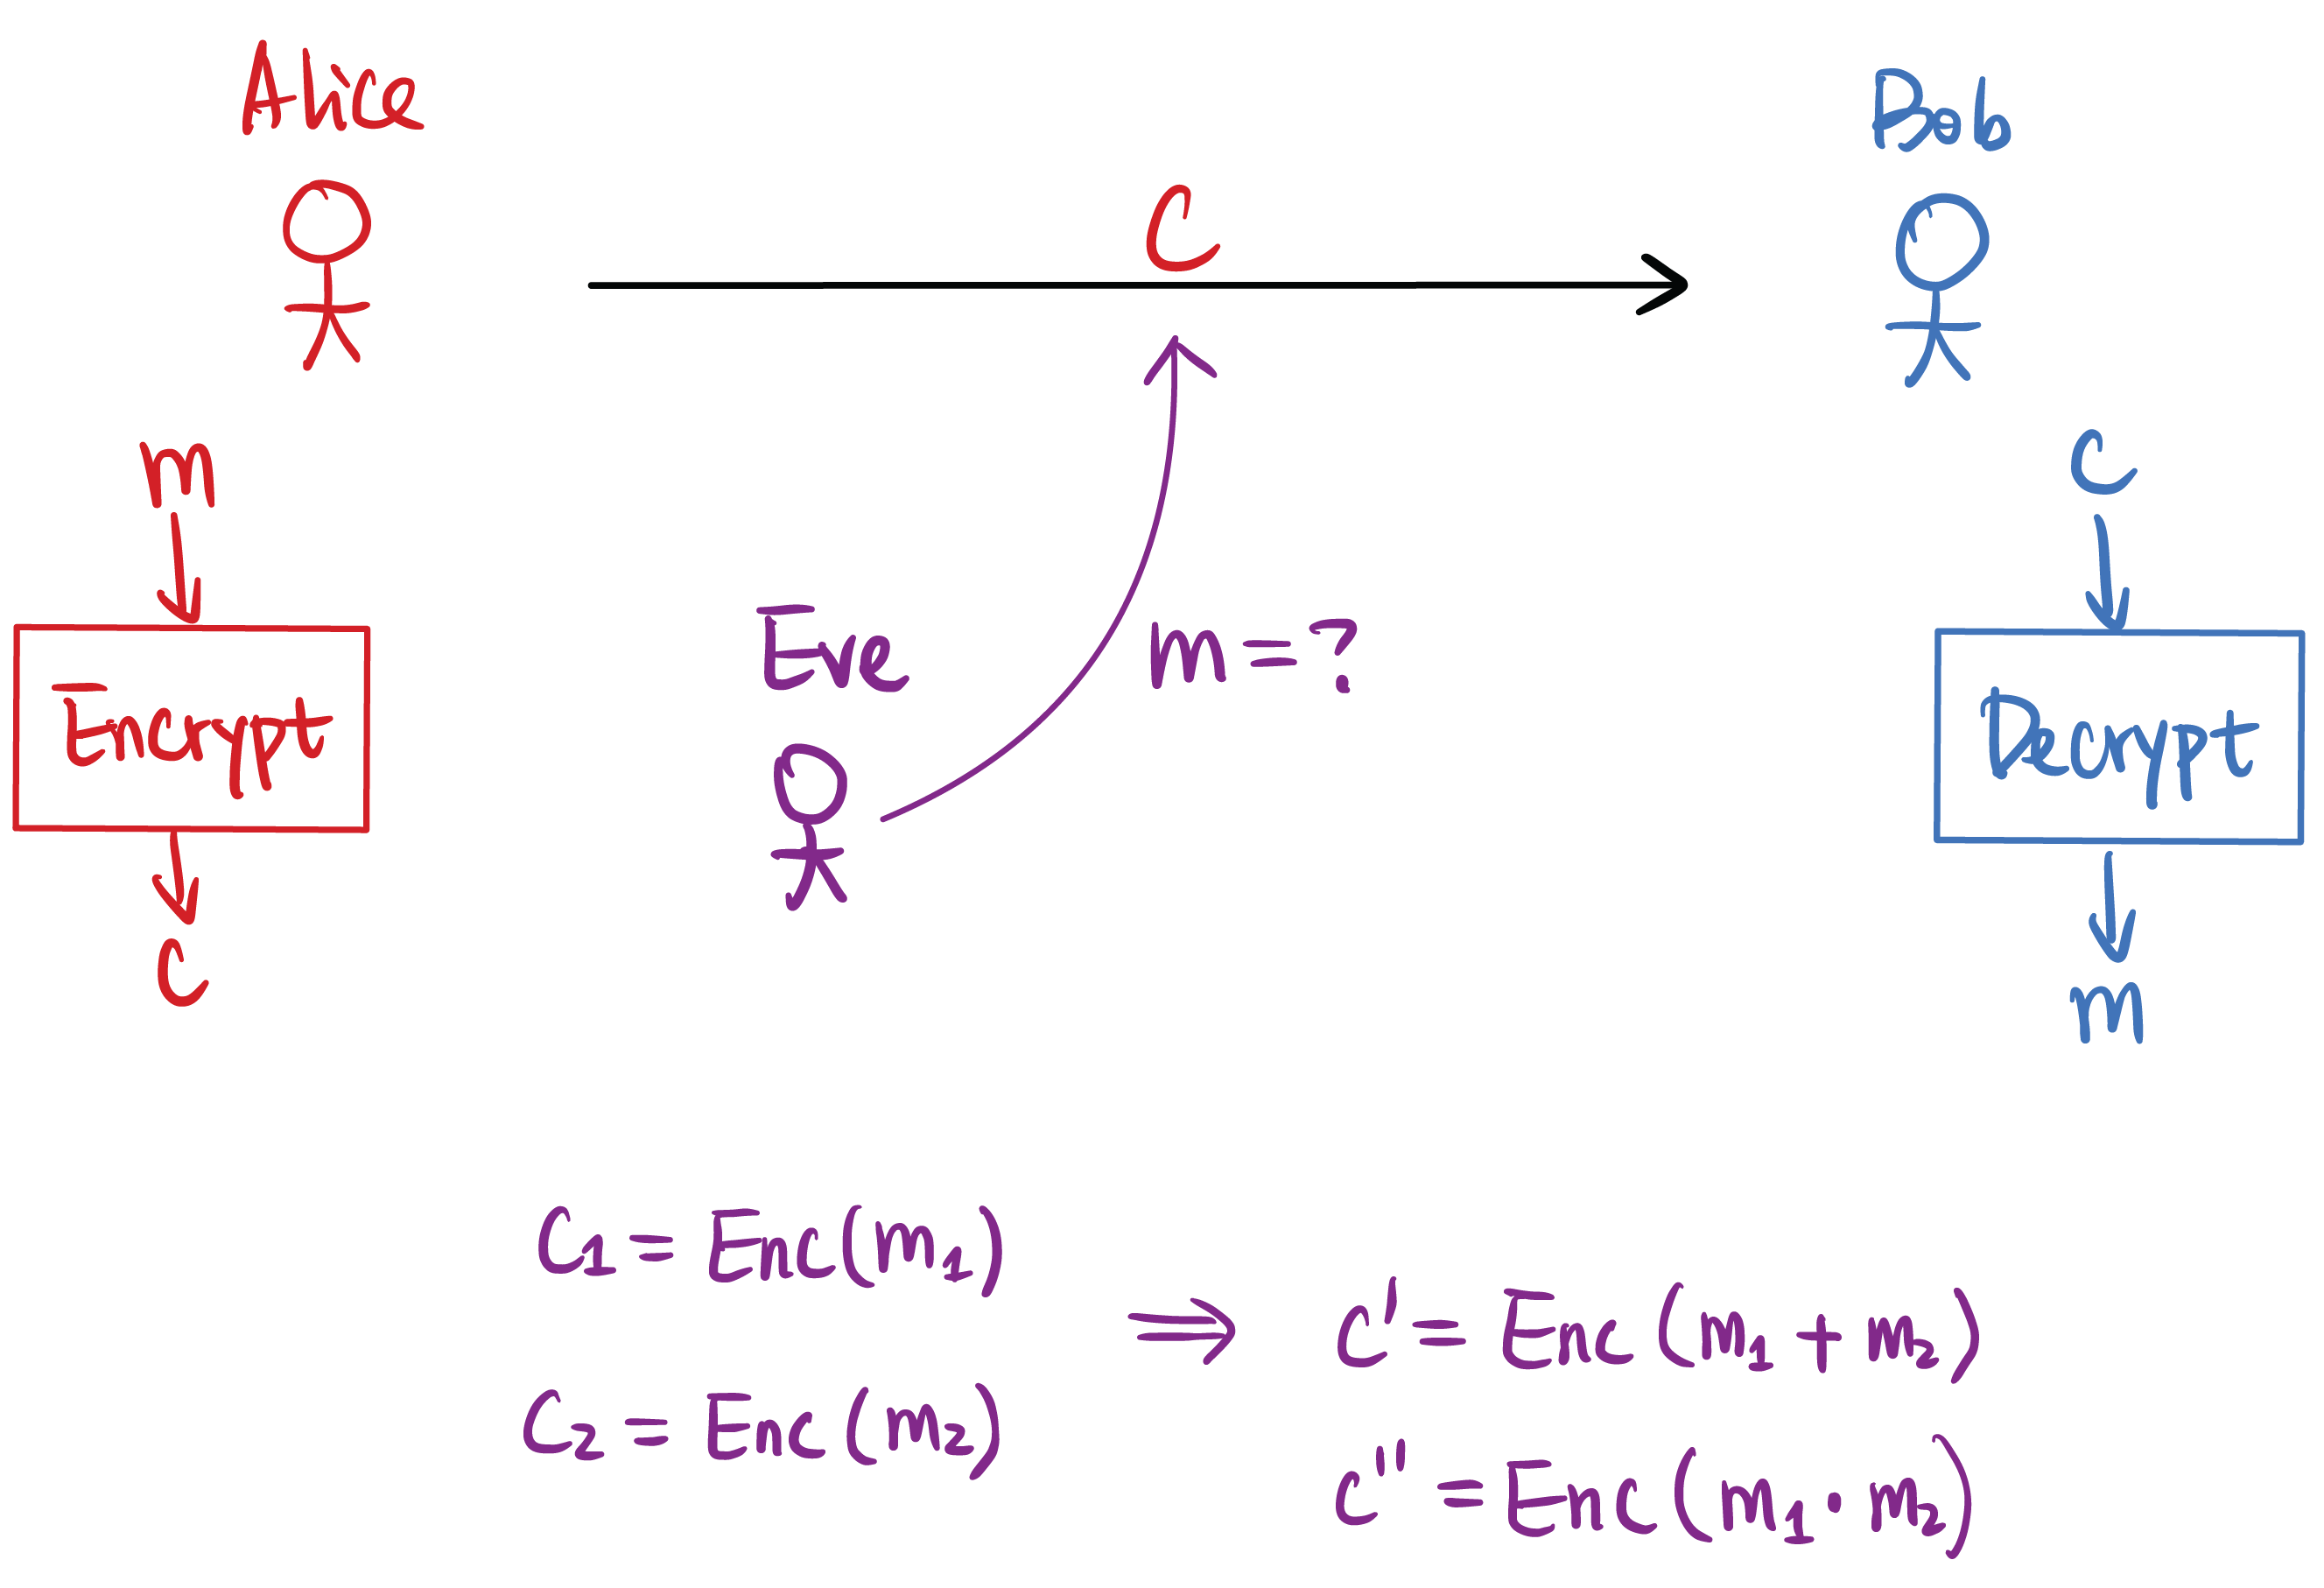
\includegraphics[width=0.9\textwidth]{images/2023-01-26/homomorphic_encryption.png}
\end{center}

We want to hopefully compute any function in polynomial time!

\begin{example*}[Outsourced Computation]
    Alice has some messages but doesn't have enough compute. There is a server that has \emph{a lot} of compute!

    \begin{center}
        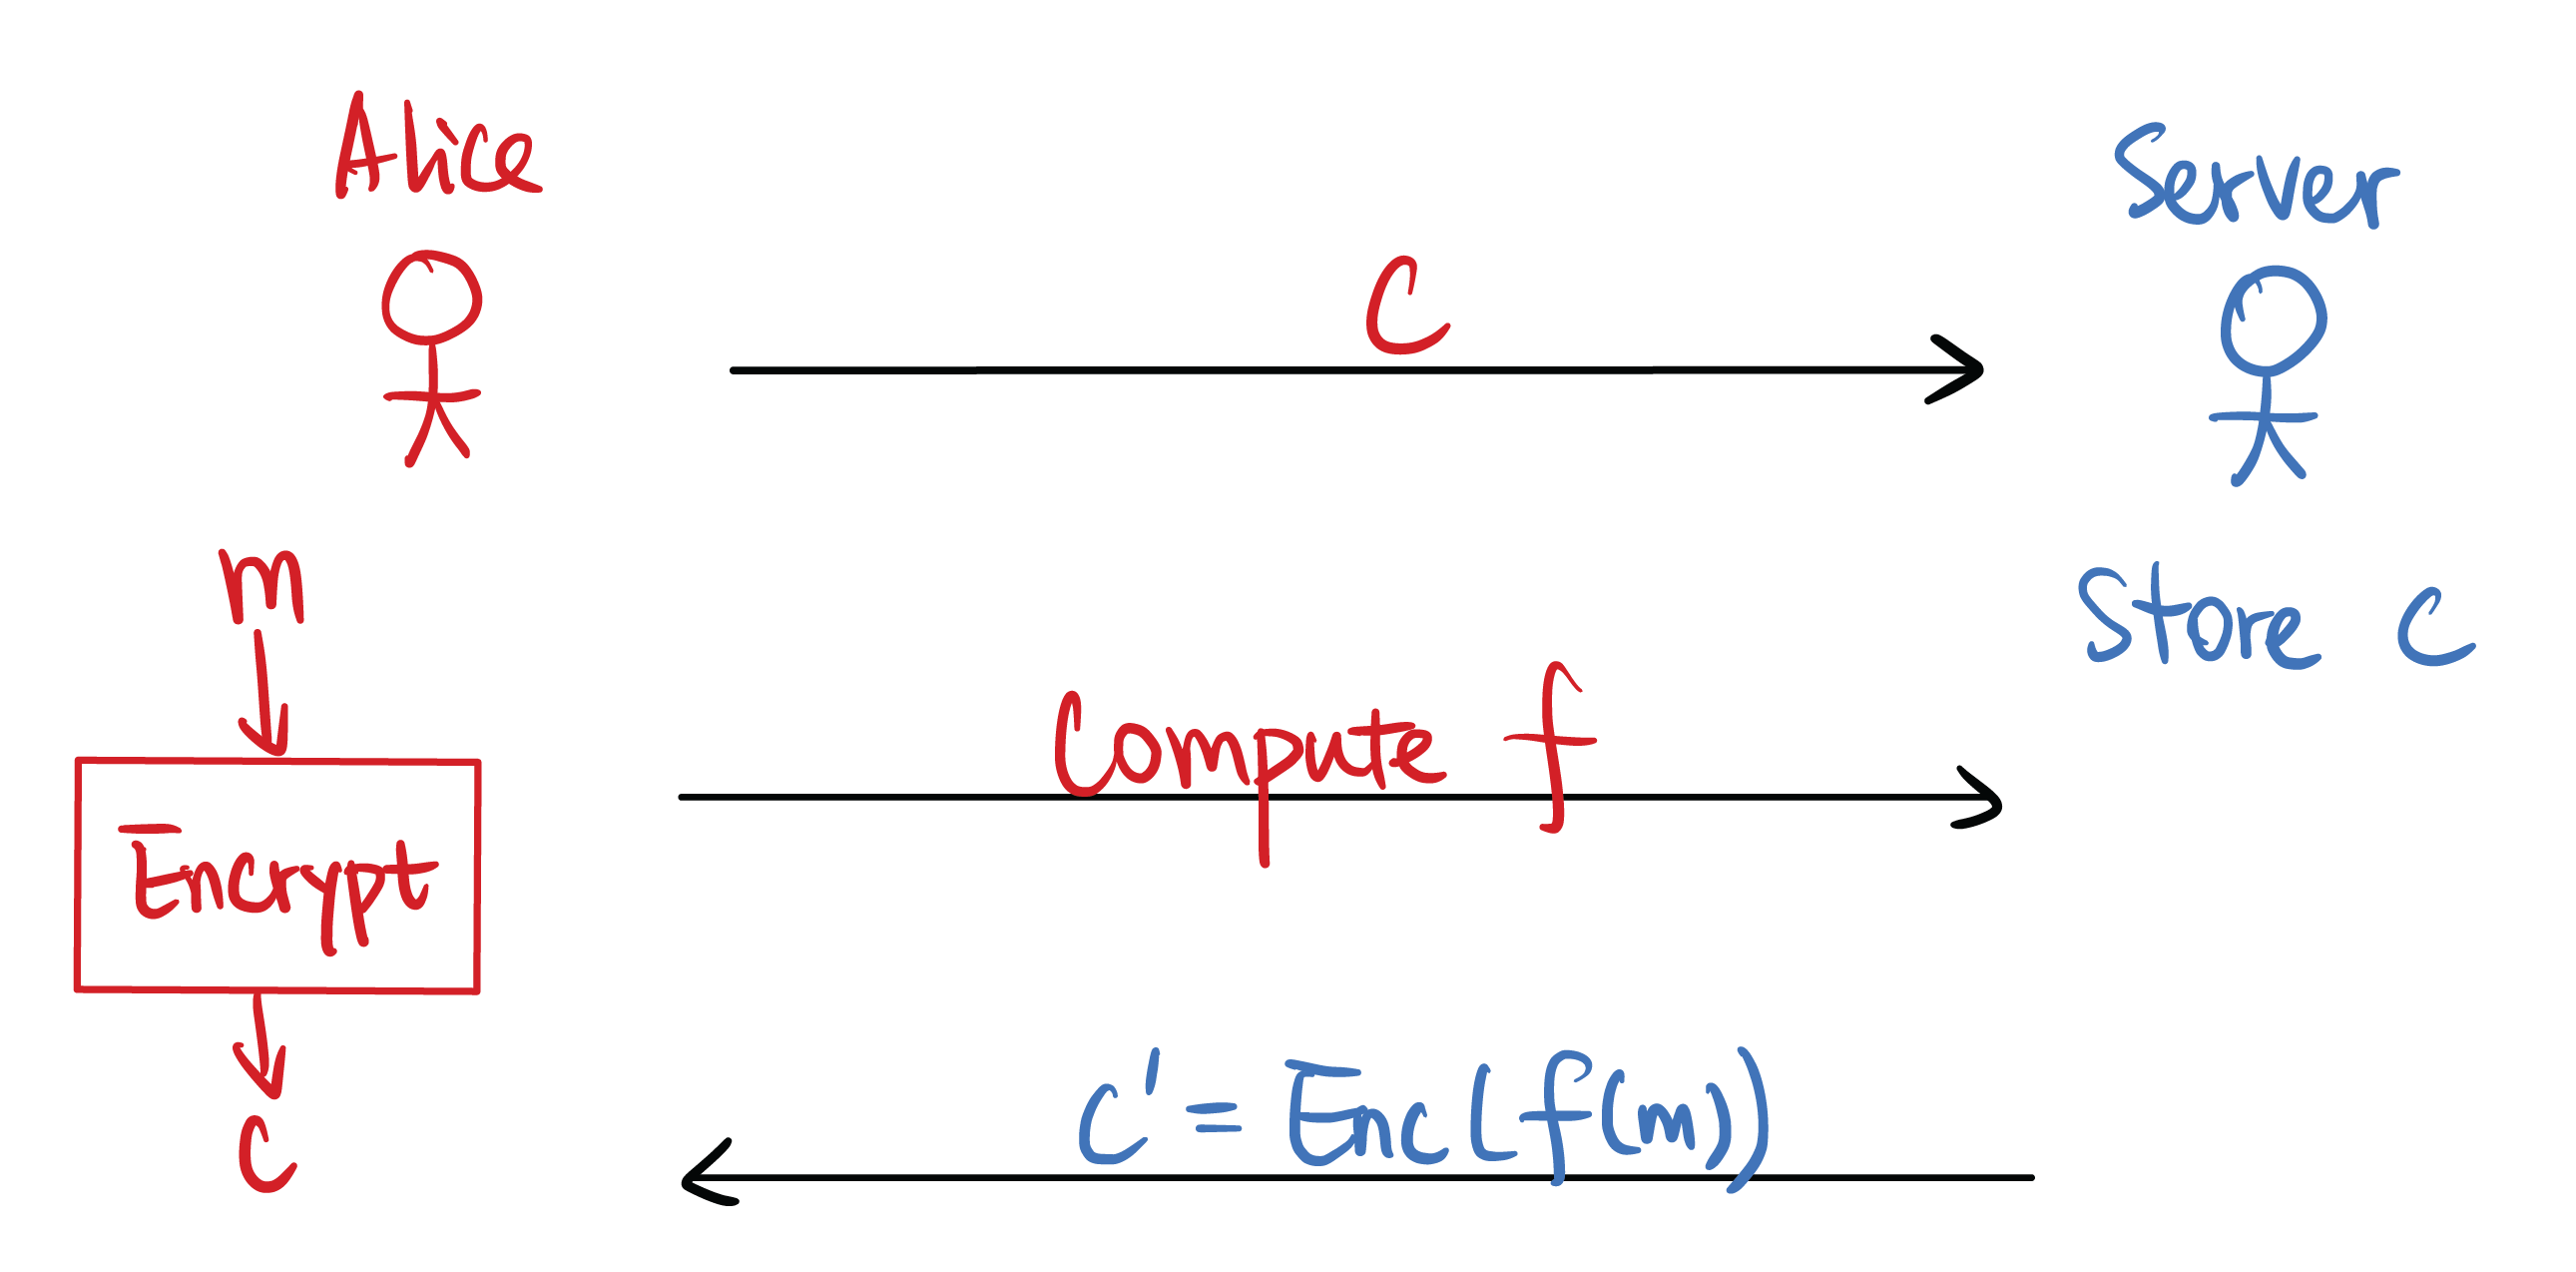
\includegraphics[width=0.9\textwidth]{images/2023-01-26/outsourced_computation.png}
    \end{center}

    Alice encrypts her data and stores it in the server. At some point, Alice might want to compute a function on the encrypted data on the server, without the server revealing the original data.

    This is an example of how fully homomorphic encryption can be useful.
\end{example*}

\begin{remark*}
    This problem was not solved until 2009 (when Peihan started her undergrad). Theoretically, it doesn't even seem that possible! Being able to compute functions on ciphertexts that correspond to functions on plaintexts.
\end{remark*}

To construct fully-homomorphic encryption, we'll be using lattice-based cryptography. This is also the only cryptographic primitive that is quantum-secure\footnote{Everything before this can be broken if quantum computers become mainstream!}.

\subsubsection{Further Topics}
We might cover some other topics:
\begin{itemize}
    \item Differential Privacy
    \item Crypto applications in machine learning
    \item Crypto techniques used in the blockchain\footnote{One important techniques is Zero-Knowledge proofs, for example.}
\end{itemize}
\emph{What else would you like to learn? What else do you want to understand?} Do go through the semester with these in mind! \emph{How do I log into Google? How do I send messages to friends?}

Peihan will collect responses at the start and middle of the semester to shape course content.

\subsection{A Quick Survey}
\emph{Peihan conducted the following poll in-class to gauge content for future lectures. \textbf{By all means, you don't need to know any/all of this going into this course! These will be self-contained in this course!}}

Do you know what the following means?
\begin{itemize}
    \item Polynomial-time algorithm.
    \item \textsf{NP}-hard problems.
    \item ``$a$ divides $b$'' ($a\mid b$)
    \item GCDs
    \item (Extended) Euclidean Algorithms
    \item Groups
    \item One-Time pads
    \item RSA encryption/signature
    \item Diffie-Hellman Key Exchange
    \item SHA (hash functions)
\end{itemize}

%!TEX root = ../notes.tex
\section{January 31, 2023}
\label{20230131}
\subsection{Logistics}
There's an EdStem post asking about topics you're interested, feel free to keep on posting!

We acknowledge the synchronization issues with Panopto. For now, if you want to watch the lecture recordings, you can use the Zoom link linked from the course home page. We can manually sync up EdStem but Panopto cannot be synced up, unfortunately.

\subsection{Encryption Schemes}
This lecture we'll cover encryption schemes. We briefly mentioned what encryption schemes were last class, we'll dive into the technical content: how we construct them, assumptions, RSA, ElGamal, etc.

Fundamentally, an encryption scheme protects message secrecy. If Alice wants to communicate to Bob, Alice will encrypt a message (plaintext) using some key which gives her a ciphertext. Sending the ciphertext through Bob using a public channel, Bob can use the key to decrypt the ciphertext and recover the message. An eavesdropper in the middle will have no idea what message has been transmitted.

\begin{center}
    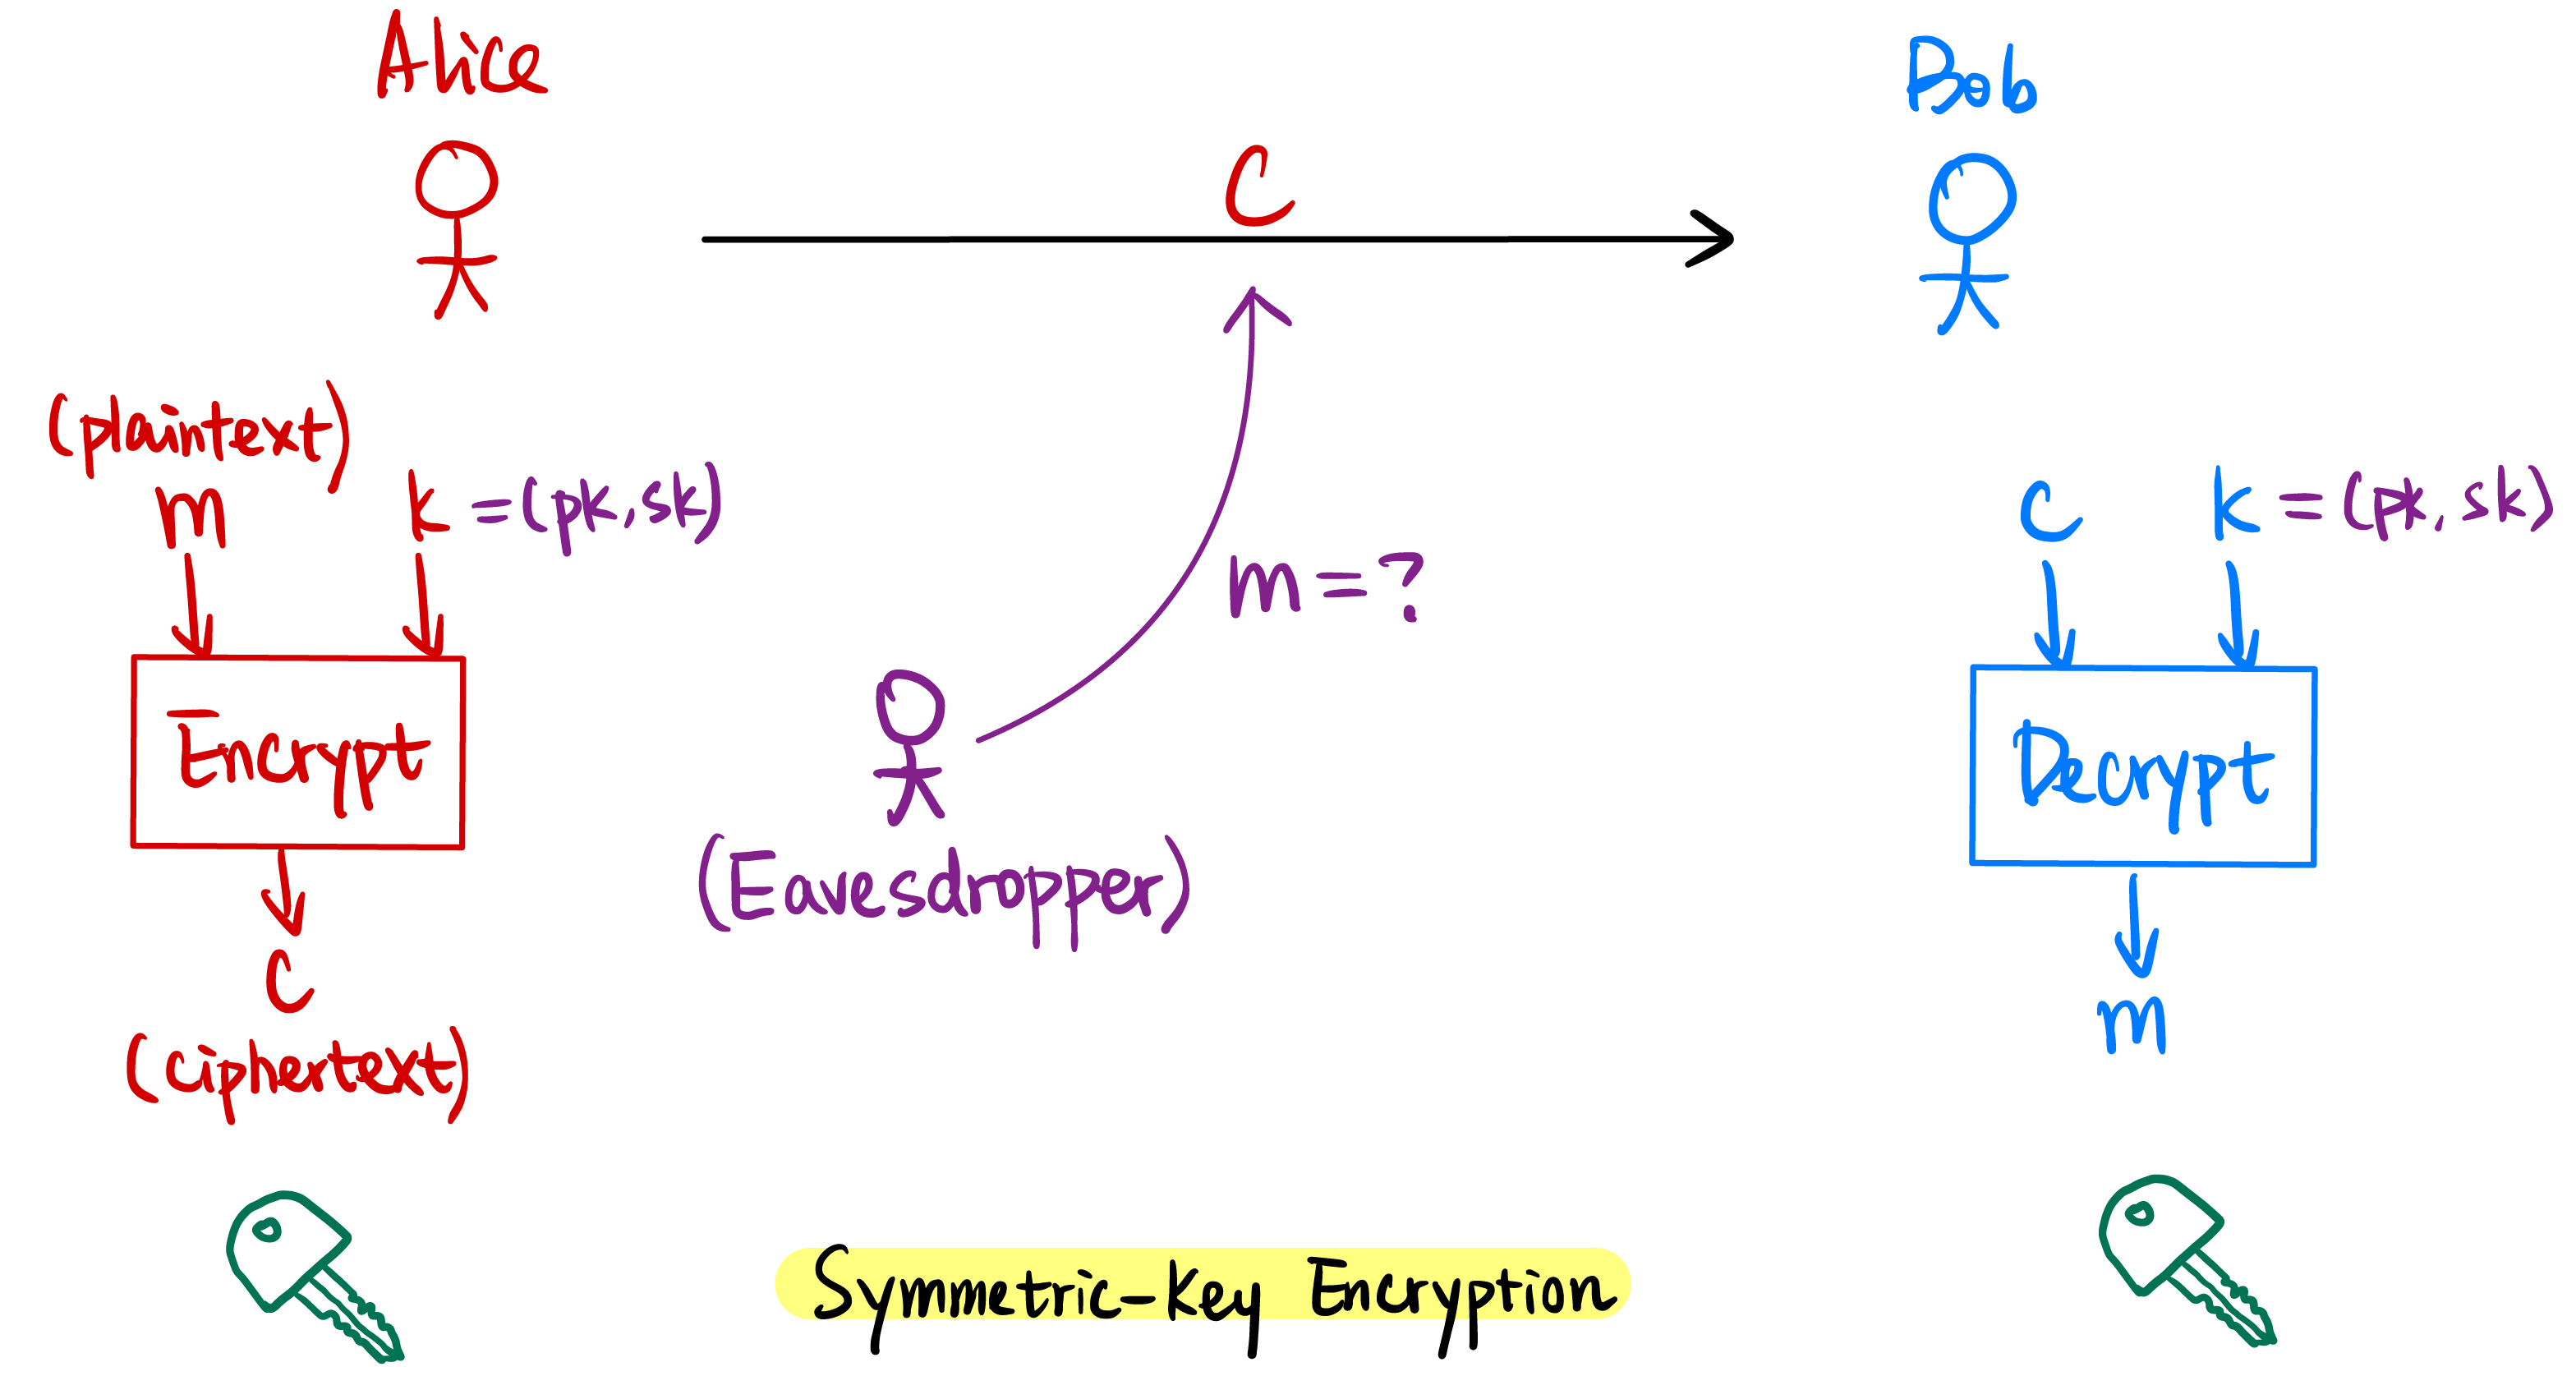
\includegraphics[width=0.8\textwidth]{images/2023-01-31/ske-intro.png}
\end{center}

In this case, they are using a shared key, which we called secret-key encryption or symmetric-key encryption.

A stronger version of private-key encryption is called public-key encryption. Alice and Bob do not need to agree on a shared secret key beforehand. There is a keypair $(pk, sk)$, a \emph{public} and \emph{private} key.

\begin{center}
    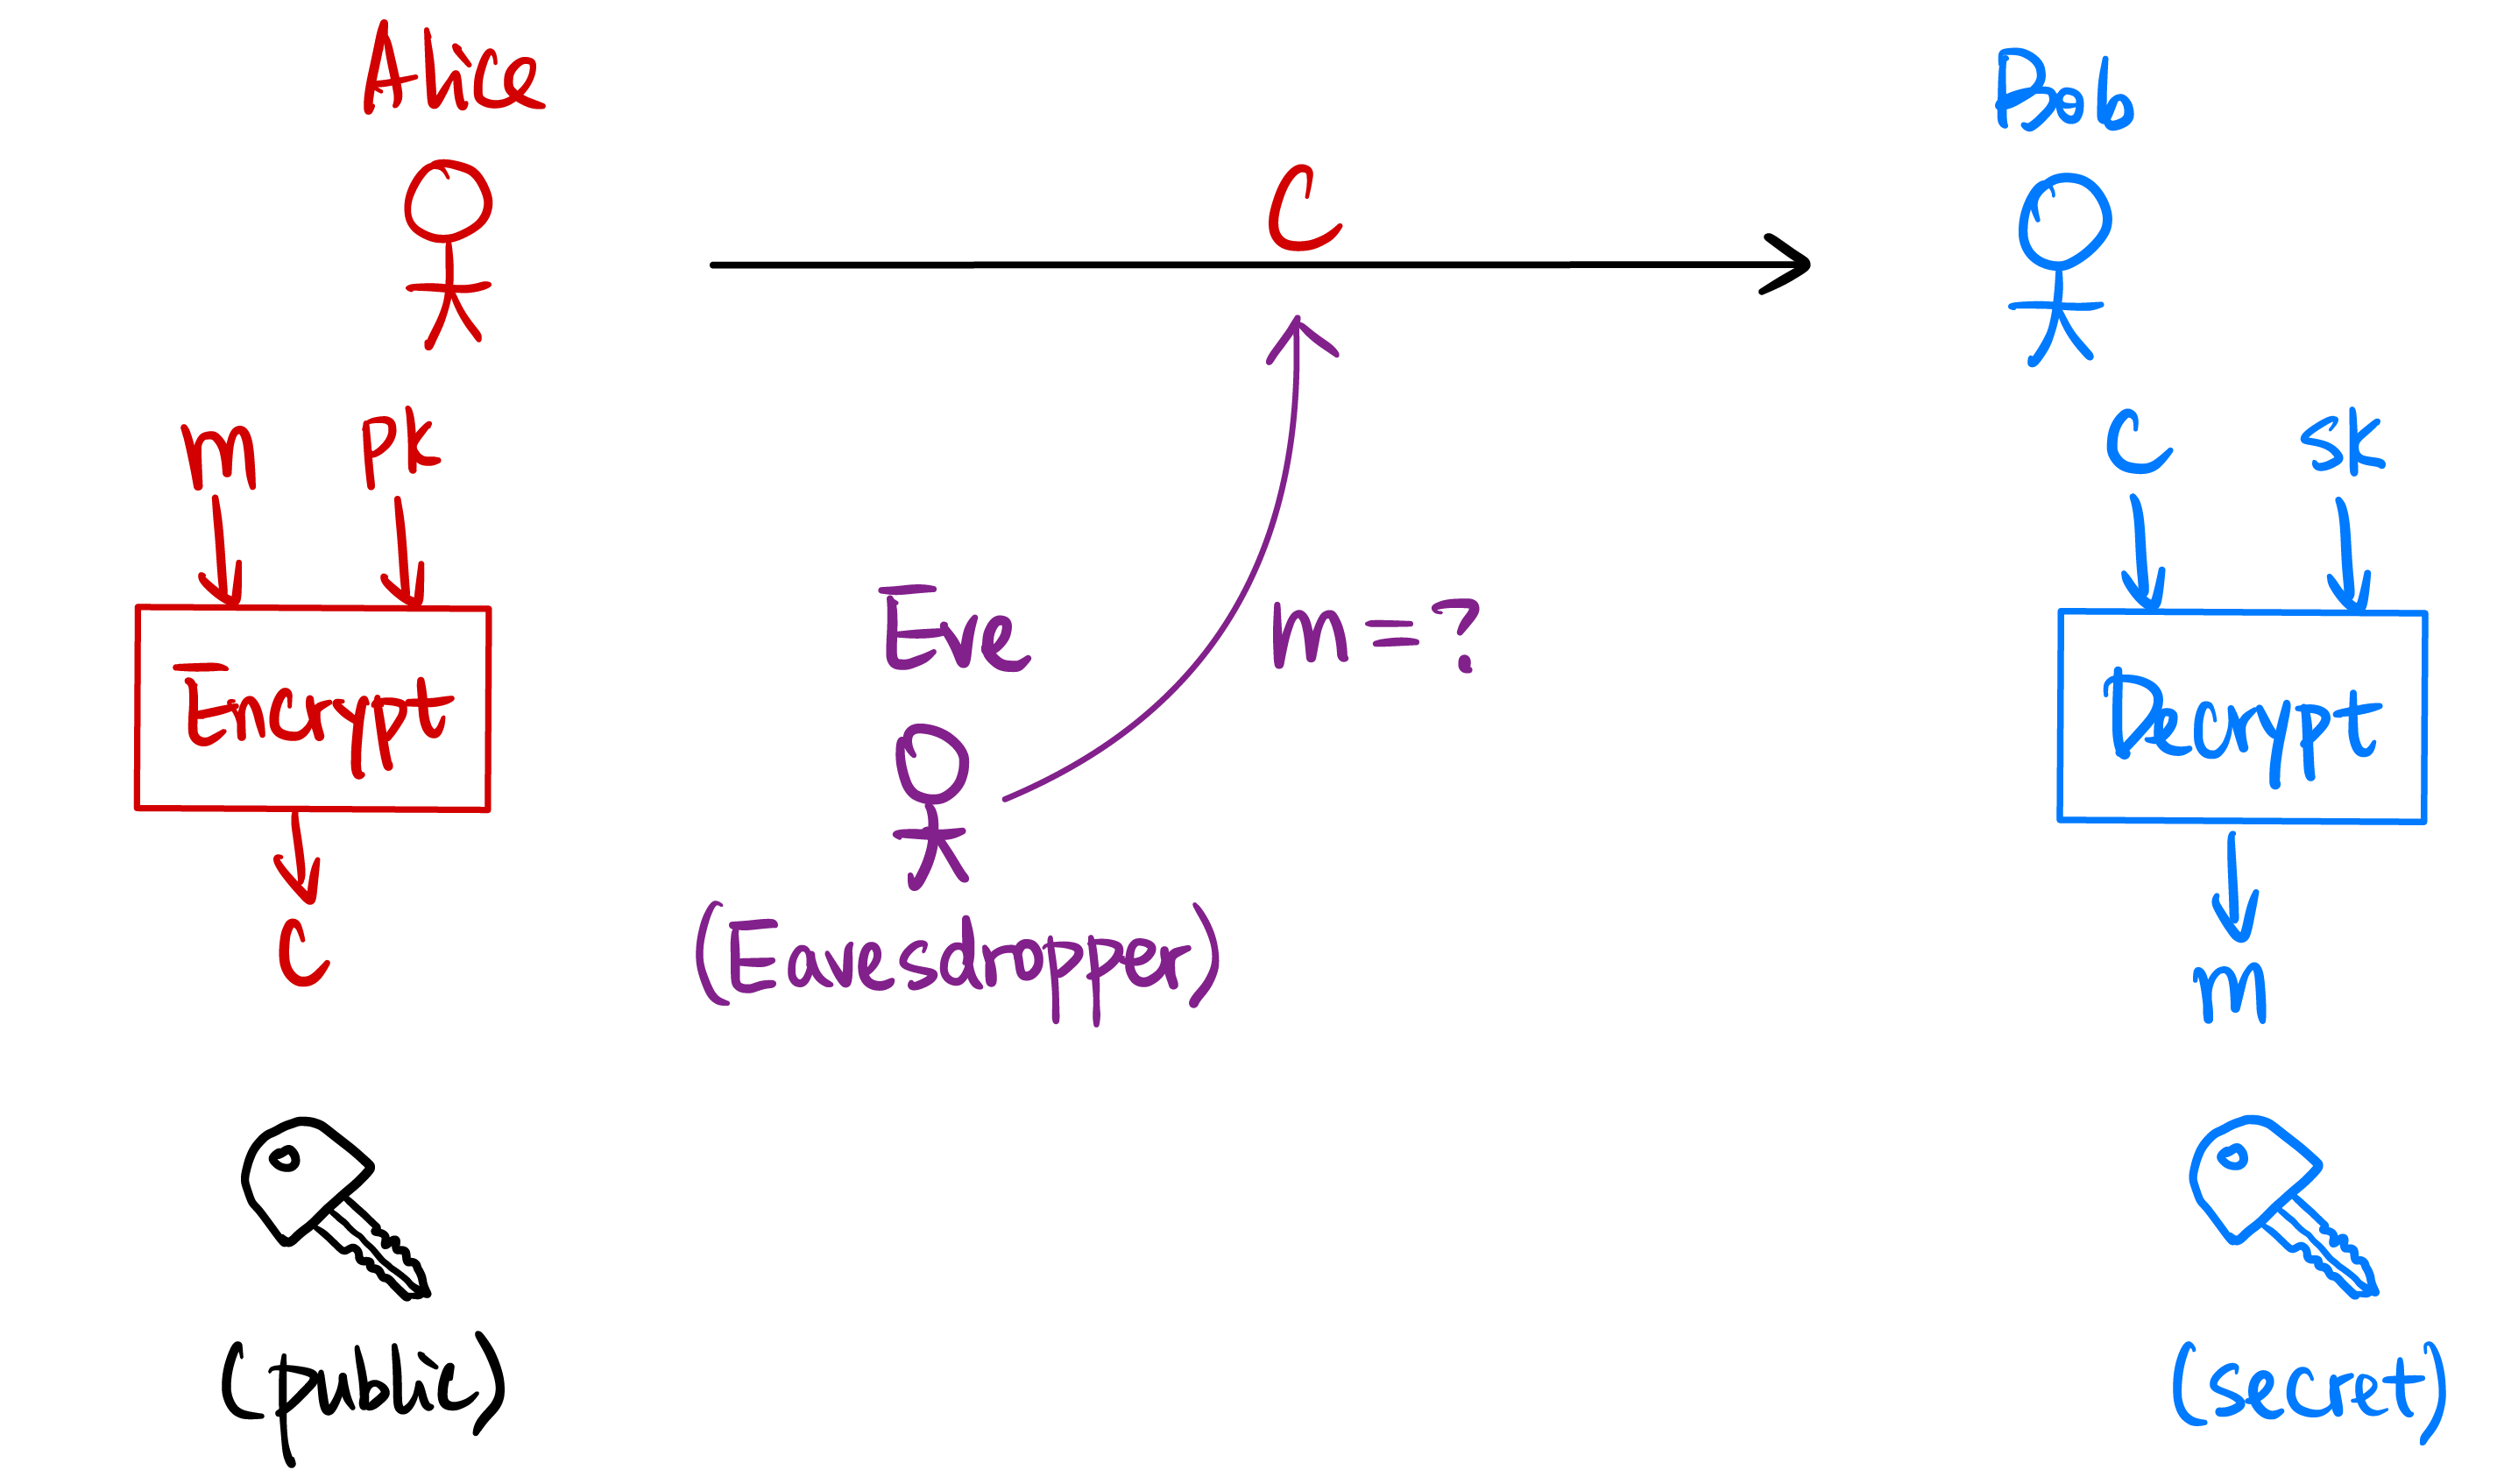
\includegraphics[width=0.8\textwidth]{images/2023-01-31/pke-intro.png}
\end{center}

\subsubsection{Syntax}
\begin{definition}[Symmetric-Key Encryption]
    A symmetric-key encryption (SKE) scheme contains 3 algorithms, $\Pi = (\mathsf{Gen}, \mathsf{Enc}, \mathsf{Dec})$.

    \begin{description}
        \item[Generation.] Generates key $k\leftarrow \mathsf{Gen}$.
        \item[Encryption.] Encrypts message $m$ with key $k$, $c\leftarrow \mathsf{Enc}(k, m)$, which we sometimes write as $\Enc_k(m)$.
        \item[Decryption.] Decrypts using key $k$ to retrieve message $m$, $m := \Dec(k, c)$, or written as $\Dec_k(c)$.
    \end{description}
    Note the notation $\leftarrow$ and $:=$ is different. In the case of generation and encryption, the produced key $k$ or $c$ follows a \emph{distribution} (is randomly sampled), but we had better want decryption to be deterministic in producing the message.
\end{definition}

\begin{definition}[Public-Key Encryption]
    A public-key encryption (PKE) scheme $\Pi = (\Gen, \Enc, \Dec)$ contains the same $3$ algorithms,

    \begin{description}
        \item[Generation.] Generate keys $(pk, sk)\leftarrow \Gen$.
        \item[Encryption.] Use the public key to encrypt, $c\leftarrow \mathsf{Enc}(pk, m)$ or $\Enc_{pk}(m)$.
        \item[Decryption.] Use the secret key to decrypt, $m:=\Dec(pk, c)$ or $\Dec_{pk}(c)$.
    \end{description}

\end{definition}

\begin{ques*}
    If we can construct public-key encryption, why do we even bother with secret-key encryption? We could just use the $(pk, sk)$ pair for our secret key, and this does the same thing.
\end{ques*}

\begin{enumerate}
    \item First of all, public-key encryption is almost always \emph{more expensive}. Symmetric-key encryption schemes give us efficiency.
    \item Public-key encryption relies on much stronger computational assumptions.
\end{enumerate}

\subsubsection{Symmetric-Key Encryption Schemes}
\begin{definition}[One-Time Pad]
    Secret key is a uniformly randomly sampled $n$ bit string $k\sampledfrom \{0, 1\}^n$.

    \begin{center}
        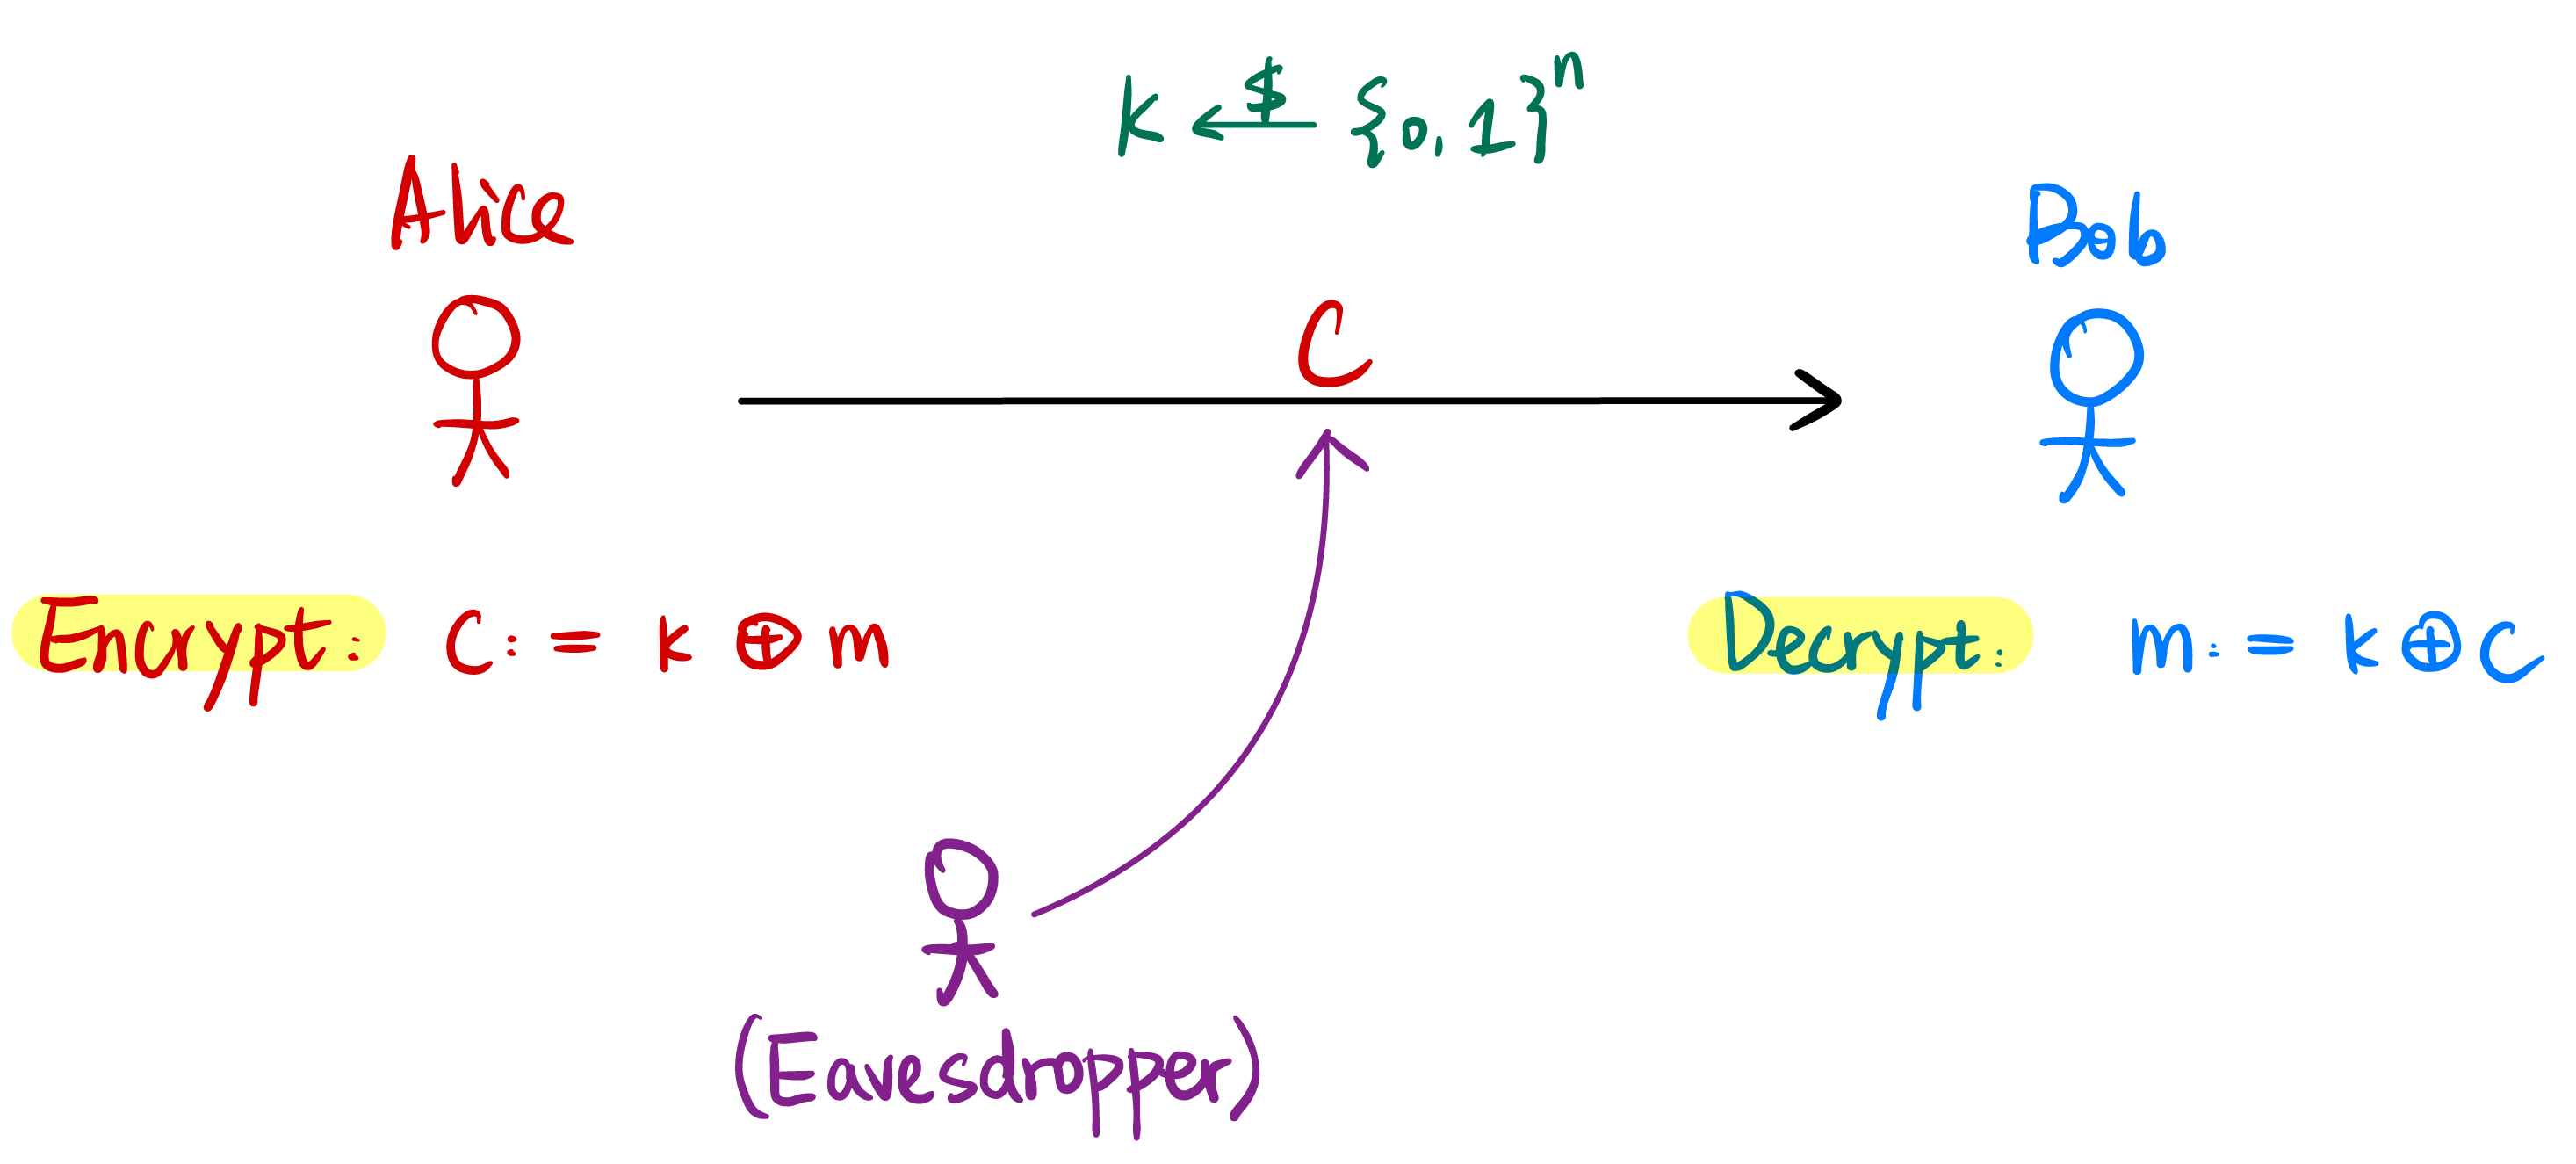
\includegraphics[width=0.7\textwidth]{images/2023-01-31/otp-defn.png}
    \end{center}

    \begin{description}
        \item[Encryption.] Alice uses the secret key and bitwise-$\mathsf{XOR}$ with the plaintext.
            \begin{align*}
                \begin{split}
                    \text{secret key}\quad k       & = 0100101 \\
                    \oplus\text{ plaintext}\quad m & = 1001001 \\ \eqline
                    \text{ciphertext}\quad c       & = 1101100
                \end{split}
            \end{align*}
        \item[Decryption.] Bob uses the secret key and again bitwise-$\mathsf{XOR}$ with the ciphertext
            \begin{align*}
                \begin{split}
                    \text{secret key}\quad k        & = 0100101 \\
                    \oplus\text{ ciphertext}\quad c & = 1101100 \\ \eqline
                    \text{plaintext}\quad c         & = 1001001
                \end{split}
            \end{align*}
    \end{description}

    This is widely used in cryptography, called \emph{masking} or \emph{unmasking}.
\end{definition}

\begin{ques*}
    Why is this correct?
\end{ques*}
An $\mathsf{XOR}$ done twice with the same choice bit $b$ is the identity. Or, an element is its own inverse with the $\mathsf{XOR}$ operator.

\begin{ques*}
    Why is this secure?
\end{ques*}

We can think about this as the distribution of $c$. $\forall m\in \{0, 1\}^n$, the encryption of $m$ is uniform over $\{0, 1\}^n$ (since $k$ was uniform).

Another way to think about this is that for any two messages $m_0, m_1\in\{0, 1\}^n$, $\Enc_k(m_0)\equiv \Enc_k(m_1)$. That is, the encryptions follow the \emph{exact same} distribution. In this case, they are both uniform, but this is not always the case.

\begin{ques*}
    Can we reuse $k$? Should we use the same key again to encrypt another message? Or, it is possible for the eavesdropper to extract information.
\end{ques*}

For example, $\Enc_k(m)$ is $c:= k\oplus m$, and $\Enc_k(m')$ is $c' := k\oplus m'$. If the two messages are the same, the ciphertexts are the same.

By $\mathsf{XOR}$ $c$ and $c'$, we get
\begin{align*}
    c\oplus c' & = (\cancel{k}\oplus m) \oplus (\cancel{k}\oplus m') \\
               & = m\oplus m'
\end{align*}
This is why this is an \emph{one-time} pad. This is a bit of an issue, to send an $n$-bit message, we need to agree on an $n$-bit message.

In fact, this is \emph{the best} that we can do.

\begin{theorem}
    \emph{Informally,} for perfect (information-theoretic\framedfootnote{That the distributions of ciphertexts are identical, that $\Enc_k(m_0)\equiv \Enc_k(m_1)$.}) security, the key space must be at least as large as the message space.
    \[|\mathcal{K}|\geq |\mathcal{M}|\]
    where $\mathcal{K}$ is the key space and $\mathcal{M}$ is the message space.
\end{theorem}

\begin{ques*}
    How can we circumvent this issue?
\end{ques*}

The high level idea is that we weaken our security guarantees \emph{a little}. Instead of saying that they have to be \emph{exactly the same} distribution, we say that they are \emph{hard to distinguish} for an adversary with limited computational power. This is how modern cryptography gets around these lower bounds in classical cryptography. We can make \emph{computational assumptions} about cryptography.

We can think about computational security,
\begin{definition}[Computational Security]\label{def:computational-security}
    We have \ul{computational security} when two ciphertexts have distribution that cannot be distinguished using a polynomial-time algorithm.
\end{definition}

\begin{definition}[Polynomial-Time Algorithm]
    A polynomial time algorithm $A(x)$ is one that takes input $x$ of length $n$, $A$'s running time is $O(n^c)$ for a constant $c$.
\end{definition}
\begin{definition}[\textsf{NP} Problem]
    A decision problem is in \ul{nondeterministic polynomial-time} when its solution can be \emph{verified} in polynomial time.
\end{definition}
\begin{example}[Graph 3-Coloring]
    Given a graph, does it have a $3$-coloring such that no two edges join the same color? For example,

    \begin{center}
        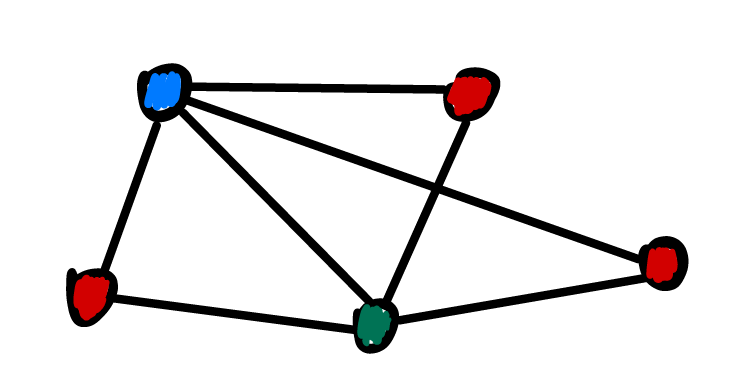
\includegraphics[width=0.4\textwidth]{images/2023-01-31/graph-coloring.png}
    \end{center}

    This can be \emph{verified} in polynomial time (we can check if such a coloring is a valid $3$-coloring), but it is computed in \textsf{NP} time.
\end{example}
\begin{definition}
    An \textsf{NP}-complete problem is a ``hardest'' problem in \textsf{NP}. Every problem in \textsf{NP} is at least as hard as an \textsf{NP}-complete problem.
\end{definition}

Right now, we assume $\mathsf{P}\neq\mathsf{NP}$. As of right now, there is no realistic algorithm that can solve any \textsf{NP} problem in polynomial-time.

Even further, we pick some problems not in $\mathsf{NP}$-complete, not in $\mathsf{P}$. We assume they are neither $\mathsf{NP}$-complete nor in $\mathsf{P}$ (we don't yet have a reduction, but we don't know if one could exist) The reasoning behind using these problems is as we have no good cryptoscheme relying solely on $\mathsf{NP}$-complete problems (we need something weaker).

\begin{center}
    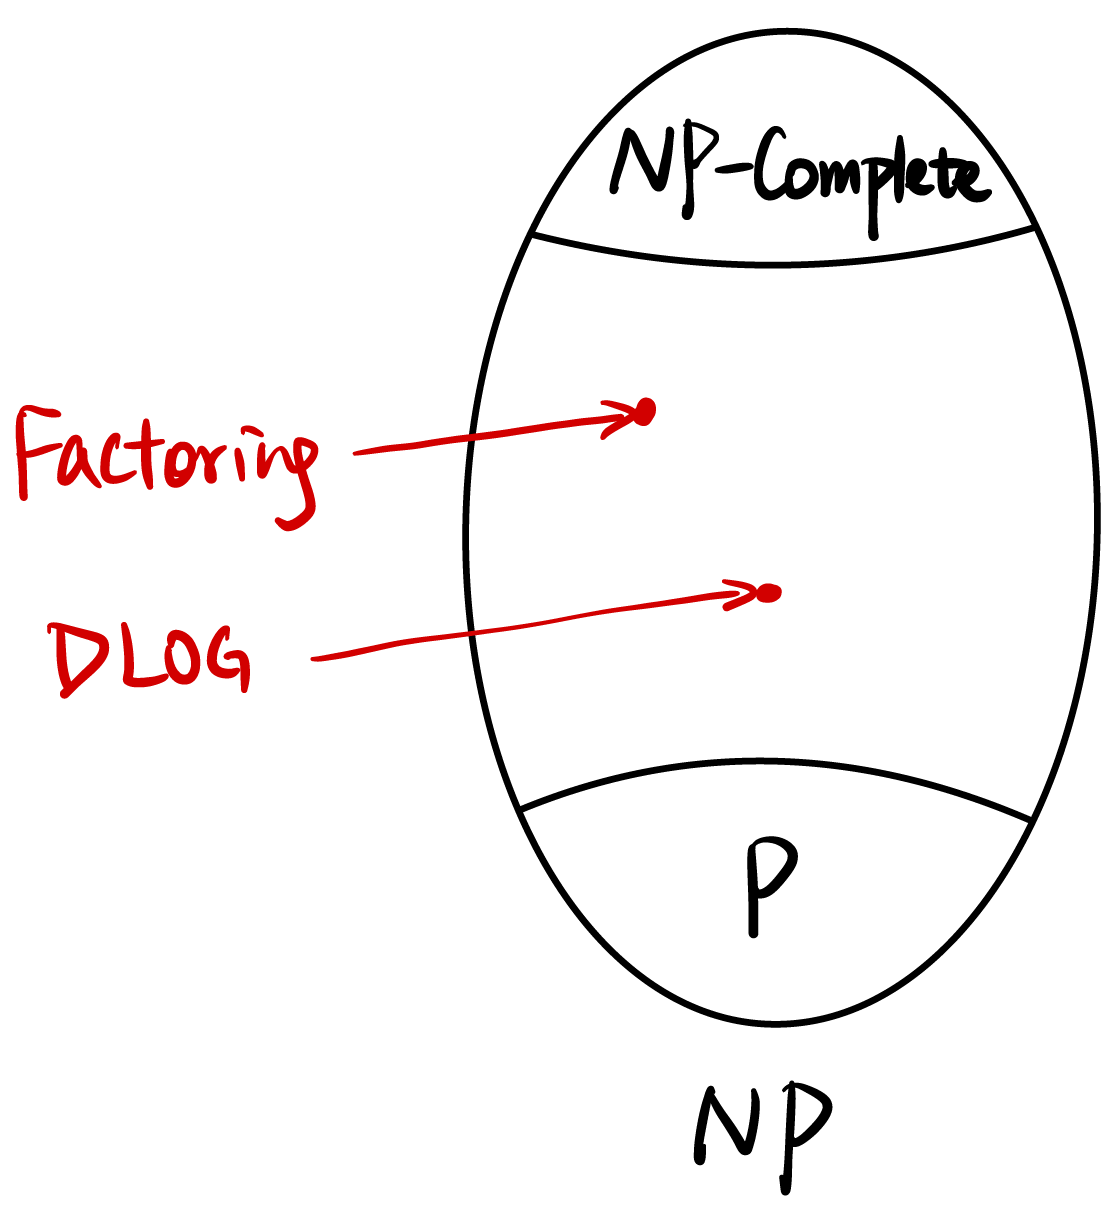
\includegraphics[width=0.4\textwidth]{images/2023-01-31/pnp-venn.png}
\end{center}

Going back to our definition of computational security \cref{def:computational-security},
\begin{definition*}[Computational Security]
    We say that the adversary is computationally bounded (is only a \emph{polynomial-time algorithm}), that $\forall \text{probabilic poly-time algorithm }\mathcal{A}$,
    \[\Enc_k(m_0)\overset{c}{\simeq}\Enc_k(m_1)\]
    Where $\overset{c}{\simeq}$ is ``computationally indistinguishable''.
\end{definition*}

What does it mean for distributions to be ``computationally indistinguishable''? Let's say Alice encrypts multiple messages $m_0, m_1, \dots$ to Bob and produces $c_0, c_1, \dots$. Even if Eve can see all plaintexts $m_i$ in the open and ciphertexts $c_i$ in the open, between known $m_0, m_1$ and randomly encrypting one of them $c\leftarrow \Enc_{k}(m_b)$ where $b\sampledfrom \{0, 1\}$, the adversary cannot determine what the random choice bit $b$ is. That is, $\Pr[b = b'] \leq \frac{1}{2} + \mathsf{negligible}(\lambda)$\footnote{$\lambda$ is the security parameter, roughly a measure of how secure the protocol is. If it were exactly equal $\frac{1}{2}$, we have information-theoretic security.}. This is Chosen-Plaintext Attack (CPA) Security.

\begin{center}
    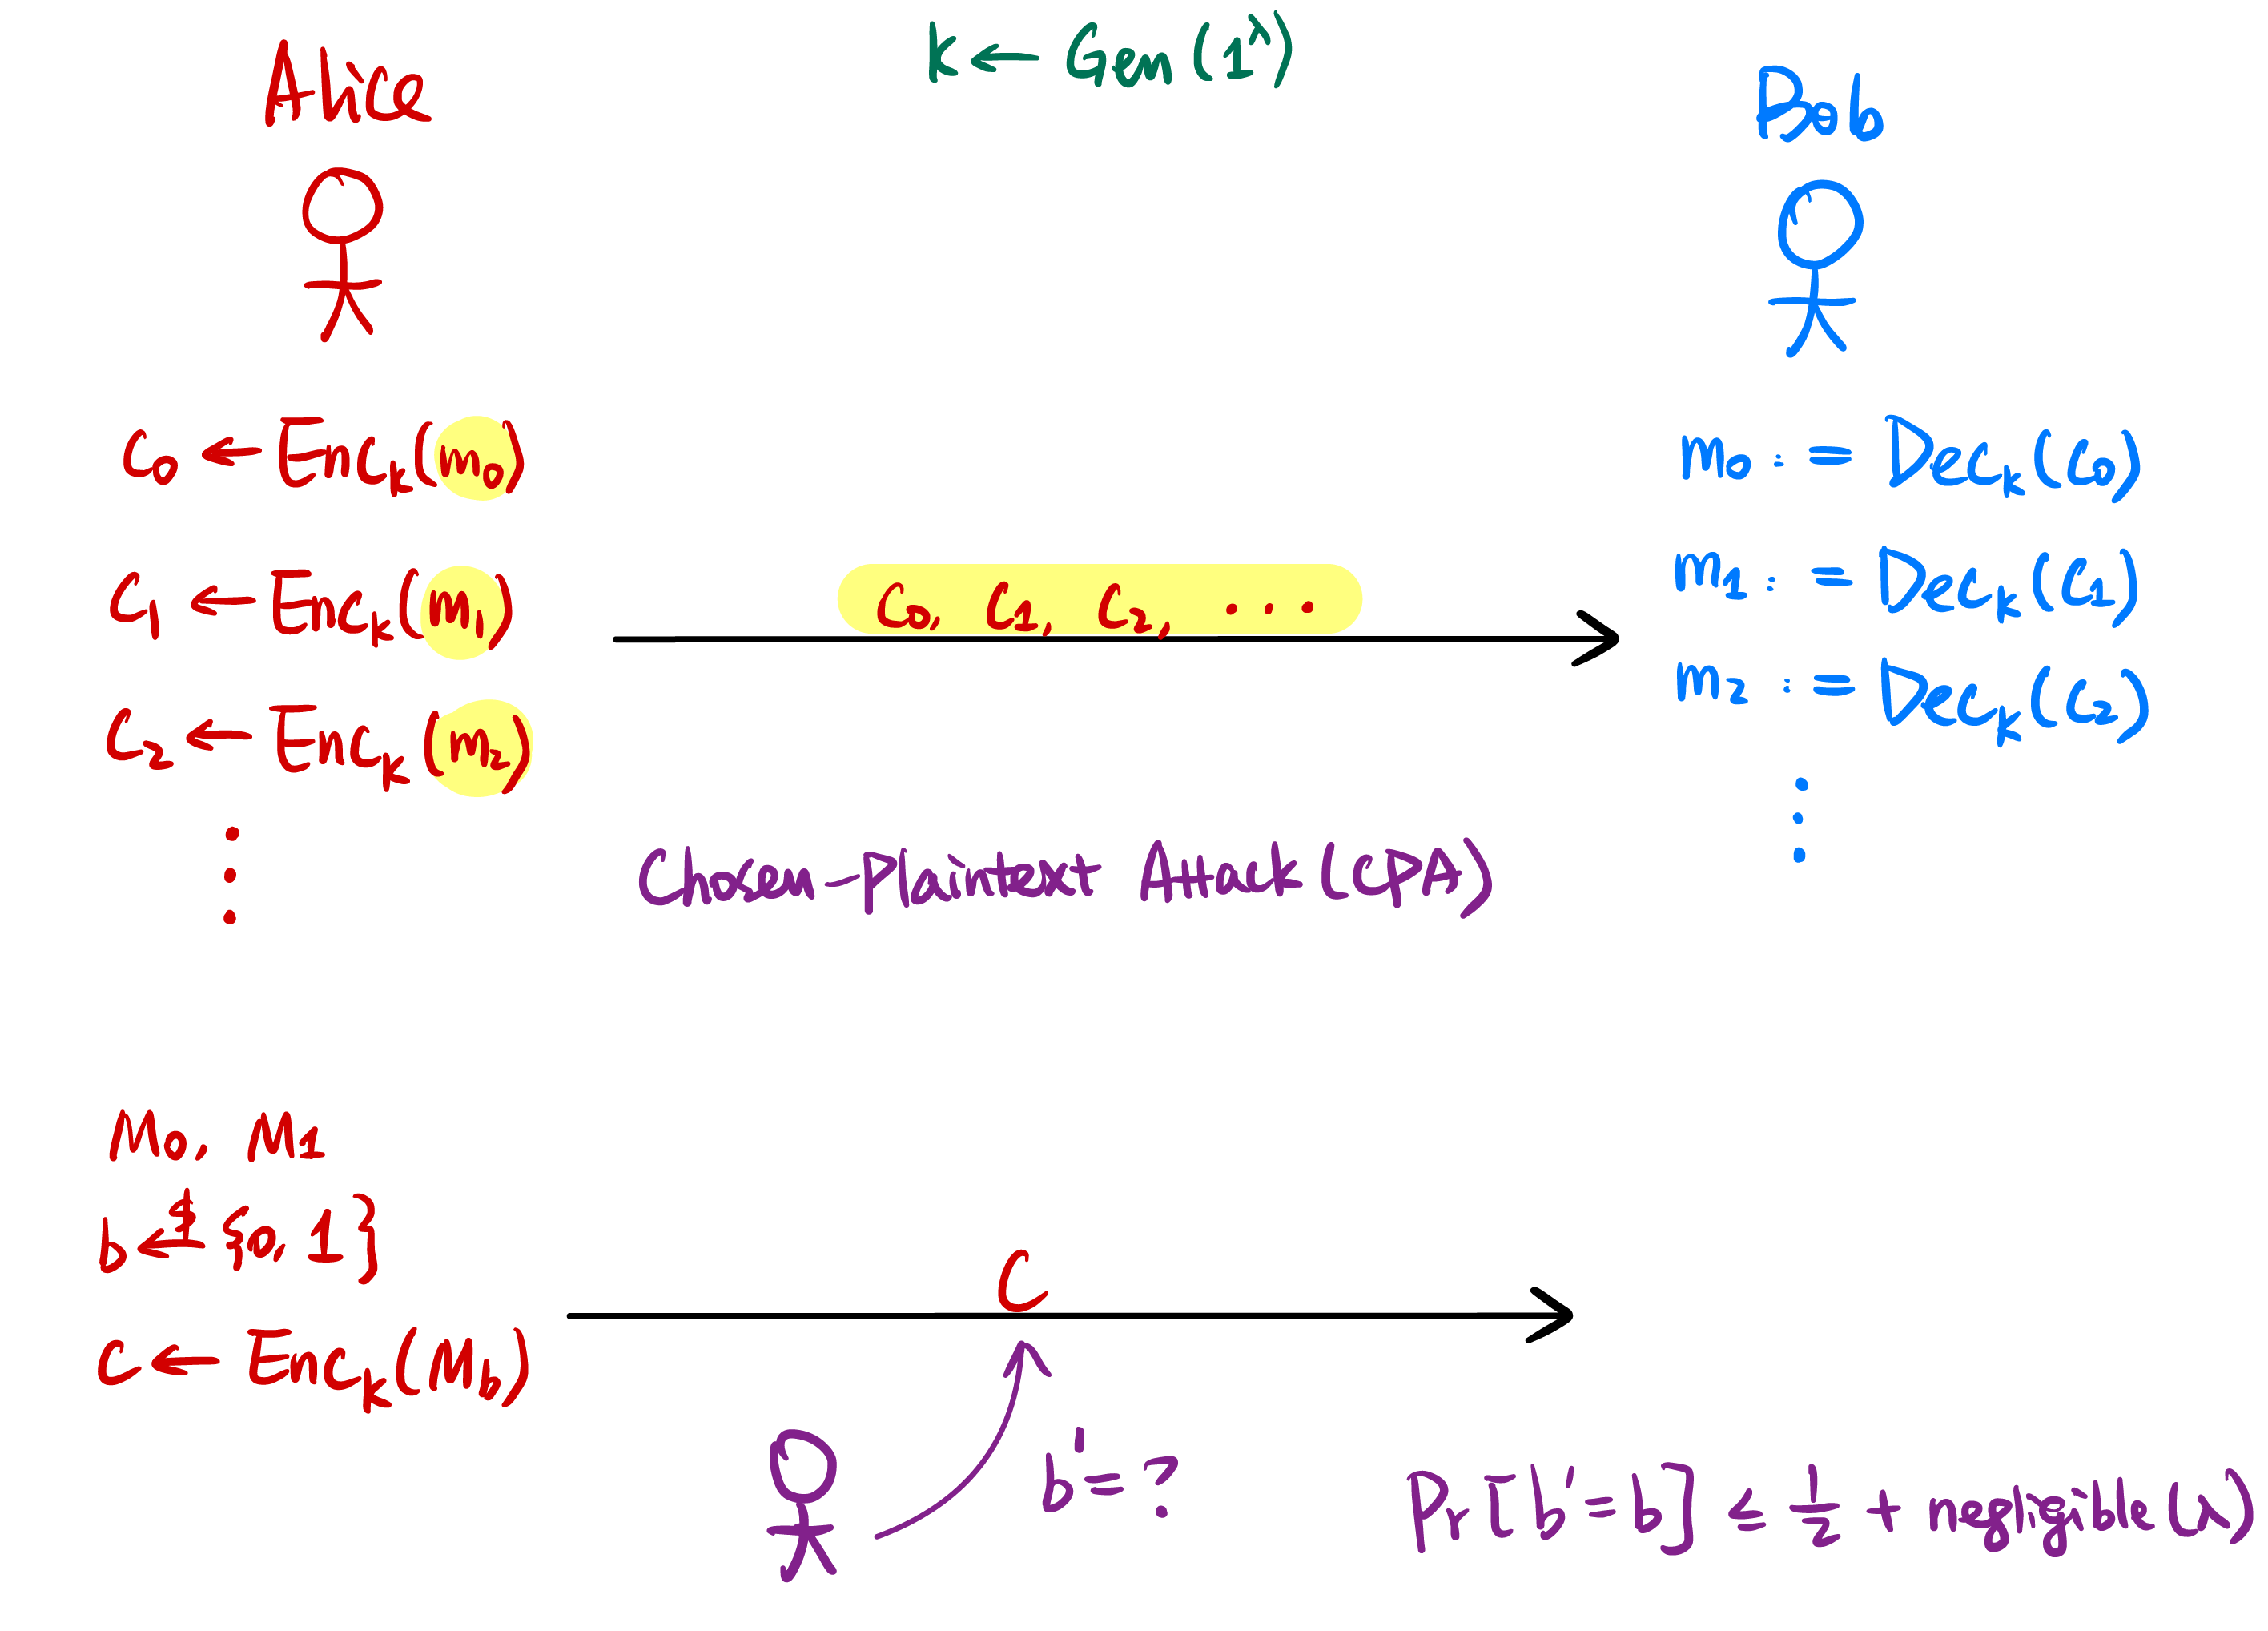
\includegraphics[width=0.8\textwidth]{images/2023-01-31/computational-security.png}
\end{center}

For a key generated $k\leftarrow \Gen(1^\lambda)$.

Theoretically, for $\lambda$ a security parameter and an adversary running in time $\mathsf{poly}(\lambda)$, the adversary should have distinguishing advantage $\negligible(\lambda)$ where
\[\negligible(\lambda) \ll \frac{1}{\lambda^c}\qquad \forall\text{ constant }c.\]

In practice, we set $\lambda = 128$. This means that the best algorithm to break the scheme (e.g. find the secret key) takes time $\sim 2^\lambda$. Currently, this is longer than the age of the universe.

\begin{example}
    \textbf{If the best algorithm is a brute-force search for $k$, what should our key length be?}

    It can just be a $\lambda$ bit string.
\end{example}
\begin{example*}
    \textbf{What if the best algorithm is no longer a brute-force search, but instead for a key length $l$ takes $\sim \sqrt{2^l}$?}

    Our key length should be $2\lambda$. Doing the math, we want $\sqrt{2^l} \equiv 2^\lambda$, solving for $l$ gives $2\lambda$.
\end{example*}

Going back to the original problem of secret-key encryption, how can we use our newfound cryptographic constructions to improve this?

From a pseudorandom function/permutation (PRF/PRP), we can reuse our secret key by passing it through the pseudorandom function.

The current practical construction for PRD/PRP is called the block cipher, and the standardized implementation is AES\footnote{Determined via a competition for such an algorithm in the early 2000s. }

It is a computational assumption\footnote{Based on heuristic, not involving any number theory!} that the AES construction is secure, and the best attack is currently a brute-force search (in both classical and quantum computing realms).

\subsubsection{Public-Key Encryption Schemes}
Using computational assumptions, we explore some public-key encryption schemes.

\begin{description}
    \item[RSA Encryption.] This is based on factoring/RSA assumption, that factoring large numbers is hard.
    \item[ElGamal Encryption.] This is based on the discrete logarithm/Diffie-Hellman Assumption, that finding discrete logs in $\ZZ_p$ is hard.
    \item[Lattice-Based Encryption.] The previous two schemes are not quantum secure. Quantum computation will break these schemes. Lattice-based encryption schemes are post-quantum secure. They are associated with the difficulty of finding `short' vectors in lattices\footnote{Covered later in class, we focus on the first two now.}.
\end{description}

Another thing worth mentioning is that
\begin{theorem}
    \emph{(Very informally,)} It is impossible to construct PKE from SKE in a black-box way. This is called ``black-box separation''.
\end{theorem}

We first need to define a bit of number-theory background.
\begin{definition}
    We denote $a\mid b$ as $a$ \ul{divides} $b$, that is, there is integer $c$ such that $b = a\cdot c$.
\end{definition}
\begin{definition}
    The $\gcd(a, b)$ is the greatest common divisor of $a, b$. If $\gcd(a, b) = 1$, then $a, b$ are coprime.
\end{definition}
\begin{ques*}
    How do we compute $\gcd$? What is its time complexity?
\end{ques*}
\begin{example*}
    We use the Euclidean Algorithm. Take $\gcd(12, 17)$,
    \begin{align*}
        17\mod{12} & = 5 \\
        12 \mod{5} & = 2 \\
        5\mod{2}   & = 1 \\
        2\mod{1}   & = 0
    \end{align*}
    or take $\gcd(12, 18)$
    \begin{align*}
        18\mod{12} & = 6 \\
        12\mod{6}  & = 0
    \end{align*}
\end{example*}
If we have two bitstrings of length $n$ bits, what is the running time of the Euclidan Algorithm?

\begin{center}
    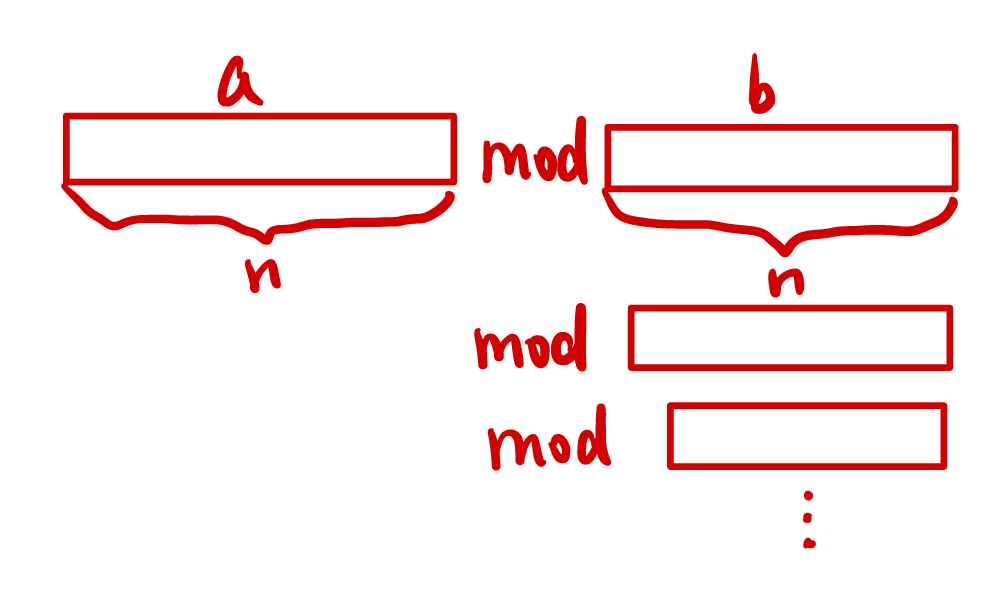
\includegraphics[width=0.3\textwidth]{images/2023-01-31/euclidean-algo.png}
\end{center}

Very informally, we see that every step, the length of $a, b$ decrease by approximately $1$ bit. Then, finding $\gcd$ is roughly order $O(n)$.

\begin{definition}[Mod]
    $a\mod{N}$ is the remainder of $a$ when divided by $N$.

    $a\equiv b\pmod{N}$ means when $a$ and $b$ are \ul{congruent modulo} $N$. That is, $a\mod N = b\mod N$.
\end{definition}

\begin{ques*}
    How might we compute $a^b\mod N$? What is the time complexity? Let $a, b, N$ be $n$-bit strings.
\end{ques*}

Na\"ively, we can repeatedly multiply. But this takes $b$ steps ($2^n$).

We can `repeatedly square'. For example, we can get to $a^8$ faster by getting $a^2$, squaring to get $a^4$, and again to get $a^8$. We can take the bitstring of $b$ and determine how to compute this.

\begin{example*}
    If $b = 100101_2$, we take $a\cdot a^4\cdot a^{32}\mod N$ which can be calculated recursively (an example is given in the first assignment).
\end{example*}

The time complexity of this is order $O(n)$ for $n$-bit $a, b, N$\footnote{Not exactly order $n$, we should add the complexity of multiplication. However, this should be bounded by $N$ since we can log at every step.}.

\begin{theorem}[Bezout's Theorem, \emph{roughly}]
    If $\gcd(a,N) = 1$, then $\exists b$ such that
    \[a\cdot b \equiv 1\pmod{N}.\]
    This is to say, $a$ is \ul{invertible modulo} $N$. $b$ is its inverse, denoted as $a^{-1}$.
\end{theorem}
\begin{ques*}
    How do we compute $b$?
\end{ques*}
We can use the Extended Euclidean Algorithm!
\begin{example*}
    We write linear equations of $a$ and $N$ that sum to $1$, using our previous Euclidean Algorithm. Take the previous example $\gcd(12, 17)$,
    \begin{align*}
        17\mod{12} & = 5 \\
        12 \mod{5} & = 2 \\
        5\mod{2}   & = 1 \\
        2\mod{1}   & = 0
    \end{align*}
    We write this as
    \begin{align*}
        5 & = 17 - 12\cdot 1                         \\
        2 & = 12 - 5\cdot 2 = 12\cdot x + 17\cdot y  \\
        1 & = 5 - 2\cdot 2 = 12\cdot x' + 17\cdot y'
    \end{align*}
    where we substitute the linear combination of $5$ into $5$ on line $2$, substitute linear combination of $2$ into $2$ on line $1$, each producing another linear combination of $12, 17$.

    If $\gcd(a, N) = 1$, we use the Extended Euclidean Algorithm to write $1 = a\cdot x + N\cdot y$, then $1\equiv a\cdot x\pmod{N}$.
\end{example*}

\begin{definition}[Group of Units mod $N$]
    We have set
    \[\ZZ_N^\times:= \left\{ a\mid a\in [1, N-1], \gcd(a, N) = 1 \right\}\]
    which is the group of units modulo $N$ (they are units since they all have an inverse by above).
\end{definition}
\begin{definition}[Euler's Phi Function]
    Euler's phi (or totient) function, $\phi(N)$, counts the number of elements in this set. That is, $\phi(N) =  |\ZZ_N^\times|$.
\end{definition}
\begin{theorem}[Euler's Theorem]
    For all $a, N$ where $\gcd(a, N) = 1$, we have that \[a^{\phi(N)} \equiv 1\pmod{N}.\]
\end{theorem}

With this, we can start talking about RSA.

\subsubsection{RSA}
We first define the RSA assumption.
\begin{definition}[Factoring Assumption]
    Given two $n$-bit primes $p, q$, we compute $N = p\cdot q$. Given $N$, it's computationally hard to find $p$ and $q$ (classically).
\end{definition}
\begin{definition}[RSA Assumption]
    Given two $n$-bit primes, we again compute $N = p\cdot q$, where $\phi(N) = (p-1)(q-1)$. We choose an $e$ such that $\gcd(e, \phi(N)) = 1$ and compute $d \equiv e^{-1}\pmod{\phi(N)}$.

    Given $N$ and a random $y\sampledfrom \ZZ_{N}^\times$, it's computationally hard to find $x$ such that $x^e\equiv y\pmod{N}$.

    \begin{center}
        
\includegraphics[width=0.4\textwidth]{images/2023-01-31/rsa.png}
    \end{center}

    However, given $p, q$, it's easy to find $d$. We know $\phi(N) = (p-1)(q-1)$, so we can compute $d$ from $e$ by running the Extended Euclidean Algorithm. Then, taking $(x^e)^d\equiv x^{ed}\equiv x$ which allows us to extract $x$ again.
\end{definition}

Encrypting is exactly raising by power $d$, and decrypting is raising again by power $e$.

Remaining questions:
\begin{itemize}
    \item How can we generate primes $p, q$?
    \item How can we pick $e$ such that $\gcd(e, \phi(N)) = 1$?
    \item What security issues can you see?
\end{itemize}

We'll continue next class.

\end{document}